%_____________________________________________________________________________________________
% LATEX Template: Department of Computer Science & Engineering MTech Seminar Reports
% Main Report
%_____________________________________________________________________________________________

\documentclass[a4paper,14pt,onecolumn]{report}

%_____________________________________________________________________________________________
% Inclusion of Required Packages
%_____________________________________________________________________________________________
\usepackage{graphicx}
\usepackage{color}
\usepackage{longtable}
\usepackage{fancyhdr}
\usepackage{setspace}
\usepackage{enumitem}
\usepackage{amsmath,amssymb,amsfonts}
\usepackage{algorithmic}
\usepackage{algorithm}
\usepackage{booktabs}
\usepackage{multirow}
\usepackage{float}
\usepackage{listings}
\usepackage{tikz}
\usetikzlibrary{positioning, arrows.meta, shapes.geometric, calc}
\usepackage{hyperref}
\hypersetup{
	colorlinks=true,
	linkcolor=black,
	citecolor=black,
	urlcolor=black
}
\usepackage{cite}

% Allow long \texttt{} paths/identifiers to break across lines and keep text in margins
\usepackage[htt]{hyphenat}
\setlength{\emergencystretch}{3em}

% Listings style for JSON / code snippets
\definecolor{codegray}{gray}{0.95}
\lstdefinestyle{snippet}{
  basicstyle=\ttfamily\footnotesize,
  backgroundcolor=\color{codegray},
  breaklines=true,
  frame=single,
  showstringspaces=false,
  columns=fullflexible,
  keepspaces=true,
}
\lstset{style=snippet}

% Graphics path for figures
\graphicspath{{figures/}{../figures/}}

%_____________________________________________________________________________________________
% Page Layout
%_____________________________________________________________________________________________
\setlength{\textwidth}{6.27in}
\setlength{\textheight}{9.69in}
\setlength{\topmargin}{0.0in}
\setlength{\oddsidemargin}{0.0in}
\setlength{\headheight}{14pt}
\setlength{\headsep}{0.2in}
\setlength{\topskip}{0.0in}

%_____________________________________________________________________________________________
% Font Definition
%_____________________________________________________________________________________________
\fontencoding{T1}
\fontfamily{cmr}
\fontseries{m}
\fontshape{n}
\fontsize{14pt}{5}
\linespread{1.5}
\selectfont

%_____________________________________________________________________________________________
% Page Numbering Style
%_____________________________________________________________________________________________
\pagestyle{fancy}
\fancyhf{}
\fancyfoot[C]{\thepage}
\renewcommand{\headrulewidth}{0pt}
\renewcommand{\footrulewidth}{0pt}

%_____________________________________________________________________________________________
% Main report starts here
%_____________________________________________________________________________________________


\begin{document}

	% ---------- FRONT MATTER ----------
	\pagestyle{empty}
	%_____________________________________________________________________________________________
% Title Page
%_____________________________________________________________________________________________

\begin{titlepage}
\begin{center}

%---------------------- Project Title ----------------------%
\LARGE{\bf{Intelligent AIOps Framework for Predictive CI/CD Pipeline Management and Autonomous Resource Optimization\\}}

\vspace{10pt}

\Large{\bf{Phase-II End-Semester Dissertation Report\\}}

\vspace{10pt}

\Large{\em{submitted by\\}}

%---------------------- Student Details --------------------%
\begin{table}[htbp]
\centering
\begin{tabular}{l c c l}
\Large\bf{Tejas Annasaheb Jagtap} &&&
\Large\bf{712442021}
\end{tabular}
\end{table}

%---------------------- Degree -----------------------------%
\LARGE{\bf{
M.Tech. Computer Science and Engineering\\
(Information Security)\\
}}

\vspace{20pt}

%---------------------- Guide ------------------------------%
\Large{Under the guidance of\\[5pt]}

\begin{tabular}{c@{\hspace{2cm}}c}
\Large{\bf{Dr. V. K. Pachghare}} & \Large{\bf{Dr. Charulata Patil}}\\
\Large{Guide} & \Large{Co-Guide}
\end{tabular}

\vspace{15pt}

\Large{COEP Technological University\\}

\vspace{10pt}

%---------------------- University Logo --------------------%
\begin{figure}[h]
\centering

\includegraphics[width=5cm,height=5cm]{NewCOEP_Logo.png}
\end{figure}

DEPARTMENT OF COMPUTER SCIENCE AND ENGINEERING

\Large{\textbf{COEP TECHNOLOGICAL UNIVERSITY}}

\vfill

June, 2026

\end{center}
\end{titlepage}

	\clearpage
	%_____________________________________________________________________________________________
% Certificate Page
%_____________________________________________________________________________________________

\thispagestyle{empty}

{
    % --- Local scope starts ---
    \linespread{1.5}\selectfont

    \begin{center}
        \LARGE\bf COEP TECHNOLOGICAL UNIVERSITY, PUNE
    \end{center}

    \begin{center}
        \large\bf DEPARTMENT OF COMPUTER SCIENCE AND ENGINEERING
    \end{center}

    \vspace{20pt}

    \begin{center}
        \Large\bf CERTIFICATE
    \end{center}

    \vspace{20pt}

    \large
    This is to certify that the Phase-II End-Semester Dissertation titled,

    \begin{center}
        \Large\bf ``Intelligent AIOps Framework for Predictive CI/CD Pipeline Management and Autonomous Resource Optimization''
    \end{center}

    has been successfully carried out and submitted by

    \begin{center}
        \Large\bf Tejas Annasaheb Jagtap \hspace{1cm} 712442021
    \end{center}

    \noindent under the guidance of \textbf{Dr. V. K. Pachghare}, in partial fulfillment of the requirements for the award of the degree of

    \begin{center}
        \textbf{Master of Technology in Computer Science and Engineering (Information Security)}
    \end{center}

    during the academic year \textbf{2025--26}.

    \vspace{130pt}

    \begin{center}
        \begin{minipage}[t]{0.48\textwidth}
            \raggedright
            \vspace{3em}
            \normalsize\bf Dr. V. K. Pachghare\\
            Guide\\
            Department of Computer Science \& Engineering\\
            COEP Technological University\\
            Pune, Maharashtra.
        \end{minipage}
        \hfill
        \begin{minipage}[t]{0.48\textwidth}
            \raggedleft
            \vspace{3em}
            \normalsize\bf Dr. P. K. Deshmukh\\
            Head of Department\\
            Department of Computer Science \& Engineering\\
            COEP Technological University\\
            Pune, Maharashtra.
        \end{minipage}
    \end{center}

} % --- Local scope ends ---

	\clearpage

	\pagenumbering{roman}
	\pagestyle{plain}

	%_____________________________________________________________________________________________
% Abstract
%_____________________________________________________________________________________________

\begin{abstract}
\addcontentsline{toc}{chapter}{Abstract}

Modern software development pipelines rely heavily on Continuous Integration and Continuous Deployment (CI/CD) systems to ensure rapid and reliable delivery. As organizations scale, these pipelines generate massive volumes of logs and highly variable workloads, making it increasingly difficult to manually detect failures, understand anomalies, and maintain optimal resource usage. Traditional monitoring tools and Kubernetes' reactive autoscaling mechanisms are often insufficient in anticipating failures or predicting future resource demands. This leads to delays, inefficient resource allocation, and increased operational overhead.

This dissertation presents the design, complete implementation, and evaluation of an intelligent AIOps-based framework that integrates machine learning into CI/CD and cloud-native infrastructure operations. The system delivers three core capabilities: (1) predicting build failures in advance using an XGBoost classifier trained on Jenkins metadata, (2) detecting anomalies in CI log streams using a TF--IDF based Autoencoder model implemented in PyTorch, and (3) forecasting future CPU usage in Kubernetes clusters through an LSTM-based time-series prediction model. These models are unified under a FastAPI-based AIOps orchestrator that loads all models at startup and serves real-time inference through REST APIs. A custom predictive autoscaler consumes these inference outputs to make proactive Kubernetes scaling decisions, replacing the reactive threshold-based behaviour of the default Horizontal Pod Autoscaler.

The complete system has been implemented and validated end-to-end. On held-out test data, the XGBoost failure-prediction model achieved 99.17\% accuracy and a 98.18\% F1-score, the TF--IDF Autoencoder anomaly detector reached 96.67\% accuracy with a 93.10\% F1-score, and the LSTM CPU forecaster attained an RMSE of 0.070 and a MAPE of 9.68\%. All three models were integrated into the orchestrator, the predictive autoscaler was implemented using the Kubernetes Python client, and the entire pipeline from data ingestion through model inference to autoscaling decisions was packaged with Docker and Kubernetes manifests. The results demonstrate the potential of AIOps to transform DevOps from reactive processes into proactive, data-driven automation.

\end{abstract}

%_____________________________________________________________________________________________

	\clearpage

	\chapter*{Acknowledgement}
\addcontentsline{toc}{chapter}{Acknowledgement}

Above all, I would like to express my sincere gratitude to my dissertation guide,
\textbf{Dr. V. K. Pachghare}, Department of Computer Science and Engineering,
for providing invaluable guidance, continuous encouragement, and unwavering support
throughout the course of this dissertation. His insightful suggestions, technical expertise,
and constant motivation greatly contributed to the successful completion of this work.

I am equally grateful to my co-guide, \textbf{Dr. Charulata Patil}, for her valuable
guidance, insightful feedback, and constant support throughout this dissertation.
Her suggestions and encouragement played an important role in shaping and refining
this work.

I would also like to express my heartfelt gratitude to
\textbf{Dr. P. K. Deshmukh},
Head of the Department of Computer Science and Engineering,
for providing an excellent academic environment and the necessary facilities to carry out this work successfully.

I extend my sincere thanks to all the faculty members, laboratory staff, administrative
staff, and non-teaching staff of the Department of Computer Science and Engineering for their support,
cooperation, and assistance throughout the dissertation work.

I am deeply grateful to my parents and family for their unconditional love, constant
encouragement, patience, and moral support, which have been a source of strength
throughout my academic journey.

I would also like to thank my friends and classmates for their valuable suggestions,
cooperation, and encouragement during the development of this work.

\vspace{2cm}

\begin{flushright}
\textbf{Tejas Annasaheb Jagtap}\\
MIS: 712442021
\end{flushright}

	\clearpage

	\tableofcontents
	\addcontentsline{toc}{chapter}{Contents}
	\clearpage

	\listoftables
	\addcontentsline{toc}{chapter}{List of Tables}
	\clearpage

	\listoffigures
	\addcontentsline{toc}{chapter}{List of Figures}
	\clearpage

	\chapter*{Keywords}
\addcontentsline{toc}{chapter}{Keywords}
AIOps, CI/CD Pipelines, Machine Learning, Failure Prediction, Log Anomaly Detection, Predictive Autoscaling, Kubernetes, XGBoost, Autoencoder, LSTM.

	\clearpage

	\chapter*{List of Abbreviations}
\addcontentsline{toc}{chapter}{List of Abbreviations}
\begin{tabular}{ll}
\textbf{AIOps} & Artificial Intelligence for IT Operations \\
\textbf{API} & Application Programming Interface \\
\textbf{AUC} & Area Under the Curve \\
\textbf{CI/CD} & Continuous Integration / Continuous Deployment \\
\textbf{CPU} & Central Processing Unit \\
\textbf{CSV} & Comma-Separated Values \\
\textbf{HPA} & Horizontal Pod Autoscaler \\
\textbf{HTTP} & Hypertext Transfer Protocol \\
\textbf{JSON} & JavaScript Object Notation \\
\textbf{LSTM} & Long Short-Term Memory \\
\textbf{MAE} & Mean Absolute Error \\
\textbf{MAPE} & Mean Absolute Percentage Error \\
\textbf{ML} & Machine Learning \\
\textbf{MSE} & Mean Squared Error \\
\textbf{RBAC} & Role-Based Access Control \\
\textbf{REST} & Representational State Transfer \\
\textbf{RMSE} & Root Mean Squared Error \\
\textbf{ROC} & Receiver Operating Characteristic \\
\textbf{SLA} & Service Level Agreement \\
\textbf{TF--IDF} & Term Frequency--Inverse Document Frequency \\
\textbf{VPA} & Vertical Pod Autoscaler \\
\end{tabular}

	\clearpage

	% ---------- MAIN CONTENT ----------
	\pagenumbering{arabic}
	\pagestyle{fancy}

%_____________________________________________________________________________________________
\chapter{Introduction}
%_____________________________________________________________________________________________

\section{Introduction to the Research Area}

Over the last decade, software development practices have undergone a major shift with the rise of DevOps, cloud-native infrastructure, and continuous automation. Modern development teams no longer depend on slow, manually executed build and deployment cycles. Instead, Continuous Integration and Continuous Deployment (CI/CD) pipelines have become the backbone of software delivery. These pipelines automatically compile code, execute tests, and deploy applications to production environments. As organizations adopt microservices, containerization, and distributed systems, CI/CD now plays an essential role in maintaining fast release cycles and ensuring product stability.

At the same time, Kubernetes has emerged as the de-facto platform for large-scale container orchestration. It manages application deployment, scaling, and resource allocation in cloud-native environments. While Kubernetes is powerful, its default automation mechanisms especially the Horizontal Pod Autoscaler (HPA) rely only on reactive rules. They respond to resource spikes after they occur rather than anticipating them.

This transformation in development and deployment workflows has created a large ecosystem of operational data. CI/CD tools like Jenkins generate thousands of log lines per build, containing warnings, test outputs, exceptions, and detailed execution traces. Prometheus captures resource usage metrics from Kubernetes clusters continuously. Developers and DevOps engineers must interpret this data to keep systems healthy, but doing so manually is increasingly impractical.

This is where the field of AIOps (Artificial Intelligence for IT Operations) has gained importance. AIOps integrates machine learning, data analytics, and automation to enhance operational decision-making. It offers capabilities like anomaly detection, real-time insight extraction, predictive analysis, and automated remediation. The research area explored in this dissertation lies at the intersection of AIOps, CI/CD intelligence, and cloud-native resource management. The core idea is to move DevOps from a reactive model to a proactive and self-learning one.

\section{Motivation for Study}

My motivation for choosing this topic comes from observing the real challenges faced by development teams working with modern CI/CD pipelines. Even with automation tools, pipeline failures often appear unexpectedly. A single unstable dependency, hidden error, or misconfigured step can cause a build to fail after running for several minutes. This wastes developer time and slows down release cycles. Many times, the root causes are buried deep within lengthy logs, making manual troubleshooting cumbersome.

Similarly, Kubernetes clusters handle highly dynamic and unpredictable workloads. Traditional autoscaling reacts to CPU or memory spikes only after the threshold is breached. This delay, even if just a few seconds, can cause service degradation, latency, timeouts, or pod failures. When teams rely heavily on microservices, these issues become even more pronounced.

From a DevOps engineer's perspective, the increasing volume of logs, metrics, and build data has become too large to analyze manually. Even experienced engineers find it difficult to track anomalies hidden within logs or predict failure-prone builds in advance. I felt that there was a strong need for an intelligent system that learns from historical patterns, continuously monitors system behavior, and takes decisions automatically.

The motivation for this dissertation, therefore, is to design and evaluate a system that integrates machine learning into CI/CD and Kubernetes operations. By analyzing pipeline history, logs, and performance data, the system aims to provide early insights that would otherwise require experienced humans to detect. The proposed solution not only benefits DevOps engineers but also contributes to higher software quality, reduced downtime, and better utilization of cloud infrastructure.

\section{Research Gaps}

Although CI/CD automation tools and Kubernetes scaling mechanisms are widely used, they still operate with significant limitations. A review of existing literature and industry practices reveals several research gaps that justify the need for this dissertation.

First, most CI/CD systems lack the ability to predict failures. They can identify problems only after they occur, often after long build processes that consume time and compute resources. The absence of predictive intelligence means that many failures especially those caused by recurring patterns or subtle anomalies could have been prevented if early warning signals were identified.

Second, log analysis within CI/CD systems is still largely reactive and manual. Logs contain rich signals about failures and unusual behavior, but due to their unstructured nature and large volume, humans cannot realistically monitor them in real time. Existing systems do not use advanced machine learning techniques like Autoencoders or Transformer-based models to detect anomalies as they occur.

Third, Kubernetes autoscaling is fundamentally reactive. Tools such as HPA depend on CPU or memory readings crossing predefined thresholds. These metrics provide no insight into upcoming workload spikes, such as developers planning to run multiple test jobs or a sudden increase in CI activity. Many studies focus either on autoscaling or log anomaly detection, but very few attempt to integrate these two domains an area that this dissertation aims to explore.

Lastly, existing research typically treats CI/CD failure prediction, log anomaly detection, and autoscaling as isolated problems. In practice, these issues are deeply interconnected. A failure in a pipeline may be caused by anomalies in logs; high workload may cause resource exhaustion; and insufficient scaling may lead to build timeouts. However, most solutions do not combine these signals into a single intelligent framework capable of responding holistically. These gaps provide a strong justification for the integrated AIOps-driven system proposed in this dissertation.

\section{Dissertation Problem Statement}

Based on the identified research gaps, the core problem addressed in this dissertation can be stated clearly as follows:

\textbf{``To design and implement an intelligent AIOps-based framework that can proactively predict CI/CD pipeline failures, detect anomalies in Jenkins logs in real time, and autonomously optimize Kubernetes resources through predictive autoscaling, thereby improving pipeline reliability, reducing operational delays, and minimizing infrastructure costs.''}

This problem focuses on replacing reactive DevOps mechanisms with proactive, data-driven decision support powered by machine learning.

\section{Research Objectives}
To address the problem statement effectively, the following research objectives were defined and have been accomplished in this dissertation:
\begin{enumerate}
    \item \textbf{Develop a Data Collection Framework for CI/CD and Cluster Metrics:} Design and implement automated data collectors that extract structured build metadata, console logs, and CPU usage metrics from Jenkins and Prometheus, and a synthetic data generator to produce training-ready datasets that mirror production CI/CD environments.

    \item \textbf{Build Machine Learning Models for Failure Prediction, Anomaly Detection, and CPU Forecasting:} Train and evaluate three ML components an XGBoost classifier for predicting CI build failures before execution, a TF--IDF based Autoencoder model for detecting anomalous log patterns, and an LSTM neural network for forecasting CPU usage trends in Kubernetes workloads.

    \item \textbf{Implement a FastAPI-Based AIOps Orchestrator for Intelligent Decision-Making:} Develop a centralized inference layer that integrates all ML models, loads them at startup, and exposes RESTful endpoints that generate actionable insights such as predicted failures, anomaly alerts, and CPU forecasts in real time.

    \item \textbf{Design a Predictive Autoscaling Engine for Kubernetes Using ML Outputs:} Create a Kubernetes-compatible autoscaler that uses ML predictions failure probability, anomaly scores, and CPU forecasts to proactively scale workloads, reduce resource wastage, and enhance CI/CD reliability, validate the complete pipeline end-to-end.
\end{enumerate}

%_____________________________________________________________________________________________
\chapter{Literature Review}
%_____________________________________________________________________________________________

\section{Detailed Literature Survey}

\begin{longtable}{|p{3.9cm}|p{2.9cm}|p{4.0cm}|p{3.4cm}|}
\caption{Detailed Literature Survey}
\label{table:lit_survey} \\
\hline
\textbf{Paper Name} & \textbf{Author(s)} & \textbf{Work Done} & \textbf{Gaps / Takeaway (Relevance to Project)} \\
\hline
\endfirsthead

\multicolumn{4}{c}{{\tablename\ \thetable{} -- continued from previous page}} \\
\hline
\textbf{Paper Name} & \textbf{Author(s)} & \textbf{Work Done} & \textbf{Gaps / Takeaway (Relevance to Project)} \\
\hline
\endhead

\hline \multicolumn{4}{r}{{Continued on next page}} \\
\endfoot

\hline
\endlastfoot

% ------------------ ROWS START ----------------------

Enhancing Machine-Learning-Based Autoscaling for Cloud Resource Orchestration~\cite{pintye2024} &
I. Pintye et al. (2024) &
Evaluates ML models for autoscaling cloud applications; compares feature sets and model architectures for predicting load and controlling scale actions. &
Focuses on autoscaling alone; lacks integration with CI/CD signals or log anomaly inputs. Does not address end-to-end AIOps orchestration across prediction, anomaly detection and scaling. \\
\hline

Time-series Forecasting-Based Kubernetes Autoscaling using Facebook Prophet and LSTM~\cite{guruge2025} &
P. B. Guruge \& Y. H. P. P. Priyadarshana (2025) &
Proposes a hybrid forecasting approach (statistical + LSTM) to predict cluster metrics and drive scaling decisions; evaluates forecast horizons and autoscale rules. &
Good forecasting results, but work evaluates autoscaling in isolation and does not incorporate CI pipeline or log features (failure predictions/anomalies). Limited discussion on real-time log integration. \\
\hline

Deep Learning for Multivariate Time-Series Anomaly Detection: A Survey~\cite{yahya2025} &
M. A. Yahya et al. (2025) &
Comprehensive survey of reconstruction-based anomaly detectors (autoencoders, VAEs, PCA, etc.) for multivariate time series; benchmarks methods and discusses thresholds. &
Survey-level work; does not present an integrated DevOps pipeline case. Guidance on thresholding useful, but lacks concrete application to text-based CI logs (TF-IDF $\rightarrow$ Autoencoder pipeline). \\
\hline

Towards Optimization of Anomaly Detection in DevOps~\cite{hrusto2023} &
A. Hrusto (2023) &
Applies deep learning techniques for detecting anomalies in monitoring and log data in DevOps contexts; experiments with representation learning and feature selection. &
Focuses mainly on monitoring metrics rather than long textual console logs; limited exploration of the combination of supervised failure prediction and unsupervised log anomaly detection. \\
\hline

AI-Enhanced Platform Engineering: Revolutionizing CI/CD Pipelines Through Intelligent Automation~\cite{das2025} &
S. Das \& P. Raj (2025) &
High-level study describing application of AI across CI/CD: predictive alerts, log triaging, and smart orchestration; includes case studies and proposed architecture patterns. &
Conceptual and high level; lacks detailed experiments, concrete model evaluation, or implementation of a closed-loop autoscaler integrating failure predictions and log anomalies.\\
\hline

Kubernetes Autoscaling with Machine Learning Based on Traffic Load Prediction~\cite{abdelhamid2025} &
Y. M. Abdelhamid, W. A. Aziz, J. N. Soliman (2025) &
Demonstrates ML-based autoscaling driven by traffic forecasts; evaluates different ML models for traffic prediction and scaling rules on Kubernetes. &
Mainly traffic-centric; does not incorporate CI/CD-specific indicators such as build queue length or log anomaly signals that are important for pipeline-aware autoscaling. \\
\hline

Predictive Failure Analysis in CI Pipelines using Ensemble Trees~\cite{mathew2025} &
R. Mathew \& S. Baswareddy (2025) &
Uses ensemble tree models (including gradient boosting) to predict CI build failures from metadata and limited log-derived features; presents feature importance analysis. &
Good match for failure prediction, but dataset size and diversity are limited; work does not combine anomaly detection or predictive scaling into a single framework. \\
\hline

LogBERT: Transformer-Based Log Anomaly Detection for CI/CD Systems~\cite{guo2021} &
H. Guo et al. (2021) &
Introduces Transformer (BERT-style) models for log representation and anomaly detection; shows improved detection of sequence-level anomalies compared with TF-IDF + Autoencoder baselines. &
High accuracy but computationally heavy; needs large labeled or pretraining corpora. Less suitable for lightweight, near-real-time deployment on small lab setups without GPUs.\\
\hline

Auto-Scaling Techniques for Container Workloads in Kubernetes Clusters A Review~\cite{sharma2025} &
P. Sharma \& R. Kumar (2025) &
Survey of HPA/VPA, custom autoscalers, rule-based vs ML-based approaches; discusses pros/cons, reactive vs predictive strategies, and common metrics used. &
Useful background material; survey highlights the need for richer signals (logs, CI metrics) but does not propose an integrated AIOps loop or evaluate combined signals. \\
\hline

Empirical Analysis on CI/CD Pipeline Evolution: Failures and Bottlenecks~\cite{houerbi2024} &
S. Houerbi et al. (2024) &
Empirical study of real-world CI/CD pipelines, identifying common failure causes, temporal patterns, and resource bottlenecks across projects. &
Descriptive study identifies problems but does not propose automated ML solutions. Useful for motivating features but lacks prescriptive integrated remediation strategies. \\
\hline

% ------------------ ROWS END ----------------------

\end{longtable}

\section{Review Summary}

The literature survey shows that existing research addresses these challenges individually, but rarely in an integrated manner. For example, Pintye et al.~\cite{pintye2024} highlight how ML-based autoscalers outperform traditional threshold-driven Kubernetes HPA, but their method relies solely on resource metrics and ignores pipeline behaviour that often drives workload changes. Similarly, Guruge and Priyadarshana~\cite{guruge2025} use Prophet and LSTM for CPU forecasting, showing promising accuracy, but their approach does not incorporate CI/CD signals or log anomalies, restricting its ability to act proactively in real-world DevOps pipelines.

In the domain of anomaly detection, Yahya et al.~\cite{yahya2025} provide a comprehensive survey of reconstruction-based deep learning models for multivariate anomalies. Their findings confirm the effectiveness of Autoencoders for identifying deviations, yet their work focuses mainly on structured system metrics rather than unstructured CI/CD logs. Meanwhile, Guo et al.'s LogBERT~\cite{guo2021} shows how transformer architectures can learn contextual log patterns more effectively than traditional models, though it demands large datasets and computation, making it less suitable for lightweight operational integration.

On the CI/CD reliability side, Mathew and Baswareddy~\cite{mathew2025} analyse build history and use ensemble models such as Gradient Boosting and XGBoost to predict failures with strong accuracy. However, the study treats CI/CD failures as isolated events rather than linking them with anomalies or infrastructure behaviour. Houerbi et al.~\cite{houerbi2024} further emphasize that many pipeline failures arise from hidden log patterns, configuration drift, and environmental inconsistencies signals that cannot be captured by metadata alone.

Across all reviewed works, the dominant research gap is that no existing system combines failure prediction, log anomaly detection, and predictive autoscaling into a unified AIOps framework. Existing solutions focus on singular parts resource metrics, logs, or build metadata leading to partial visibility. A holistic system integrating these signals could provide deeper situational awareness, more reliable pipelines, and proactive infrastructure optimisation. This gap forms the foundation of the dissertation's proposed architecture.

%_____________________________________________________________________________________________
\chapter{Proposed Methodology}
%_____________________________________________________________________________________________

\section{Overview}

The proposed AIOps-based framework integrates multiple intelligent components that work together to enhance the reliability, efficiency, and scalability of CI/CD pipelines running in cloud-native environments. Modern DevOps ecosystems consist of several interacting elements such as CI tools, log streams, monitoring systems, and Kubernetes-based deployments. Traditional approaches treat these components independently, but the increasing complexity and scale of software delivery demand a unified design that allows these systems to exchange information, learn from historical behavior, and make proactive decisions.

The high-level design of the system centers around three primary machine learning modules failure prediction, log anomaly detection, and CPU workload forecasting and a FastAPI-based orchestration layer that connects them to external systems like Jenkins, Prometheus, and Kubernetes. Rather than relying on reactive or threshold-based automation, the architecture enables the system to anticipate failures, detect anomalies in real-time, and adjust compute resources proactively. This chapter describes the major components of the architecture, their interactions, the design of the machine learning models, and the predictive autoscaling policy.

\section{System Architecture Components}

The architecture is composed of several interconnected modules, each contributing to the system's ability to perform predictive and autonomous operations.

\subsection{Jenkins Data Collection Layer}
Jenkins serves as the primary source of CI/CD pipeline information. This component retrieves build metadata such as build duration, timestamps, status labels, and test results, along with detailed console logs that capture every step in the build process. The Jenkins REST API is used to extract these records, which are then preprocessed for downstream machine learning tasks. Console logs, being unstructured, are cleaned and normalized before vectorization using TF-IDF.

\subsection{Prometheus Metrics Collector}
Prometheus acts as the monitoring backend of the architecture. It collects time-series metrics from the Kubernetes cluster, including CPU utilization, memory usage, and pod replica counts. The collected data is essential for training and running the LSTM-based CPU forecasting model. The metrics are periodically fetched through the Prometheus HTTP API and stored in structured formats suitable for training.

\subsection{Machine Learning Models}
The framework integrates three ML models:

\begin{itemize}
    \item \textbf{Failure Prediction Model (XGBoost):} Trained on structured Jenkins metadata, this model predicts whether a build is likely to fail before execution. It helps reduce wasted compute time and enhances CI/CD reliability.
    \item \textbf{Log Anomaly Detection Model (Autoencoder):} Using TF-IDF vectors derived from console logs, the Autoencoder learns patterns of normal behavior. Deviations generate high reconstruction errors, allowing real-time identification of unusual or potentially hazardous log segments.
    \item \textbf{CPU Forecasting Model (LSTM):} Built using time-series metrics from Prometheus, this model forecasts CPU usage several minutes ahead. Its predictions enable proactive scaling decisions.
\end{itemize}

\subsection{FastAPI-based AIOps Orchestrator}
The orchestrator acts as the central communication hub. It loads the trained ML models into memory and exposes a set of RESTful APIs that other components can interact with. These include:

\begin{itemize}
    \item \texttt{/predict\_failure}: returns failure probability
    \item \texttt{/detect\_anomaly}: returns anomaly score and flag
    \item \texttt{/forecast\_cpu}: provides CPU forecasts
    \item \texttt{/autoscale}: triggers the predictive autoscaling engine
\end{itemize}

The orchestrator ensures modularity, allowing models to be updated independently without altering pipeline logic.

\subsection{Predictive Autoscaler}
Traditional Kubernetes Horizontal Pod Autoscaler (HPA) performs scaling based purely on current CPU metrics. In contrast, the predictive autoscaler uses LSTM forecasts to scale resources ahead of time. It also incorporates anomaly scores and failure probabilities to avoid unnecessary scaling during unstable conditions. The autoscaler communicates with the Kubernetes API server to update replica counts and enforces constraints such as cooldown intervals, minimum/maximum replicas, and rate limits.

\section{System Architecture Diagrams}
\begin{figure}[H]
    \centering
    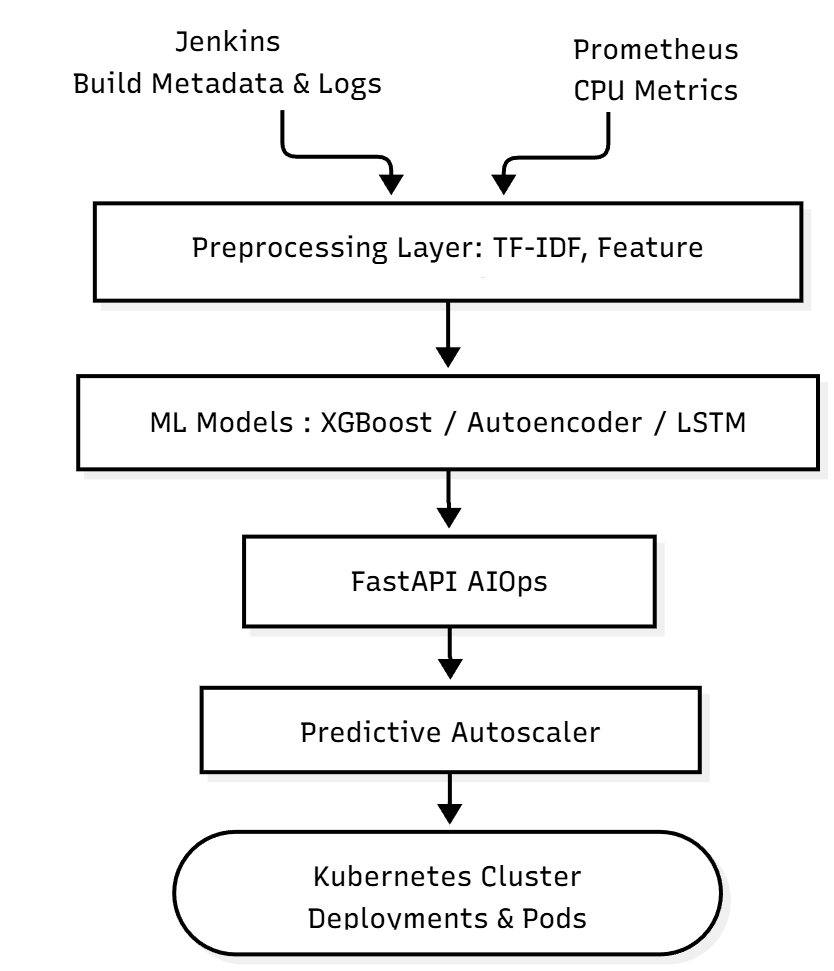
\includegraphics[width=0.70\textwidth]{overview.png}
    \caption{Overall Overview of the Proposed AIOps System}
    \label{fig:system_overview}
\end{figure}

\begin{figure}[H]
    \centering
    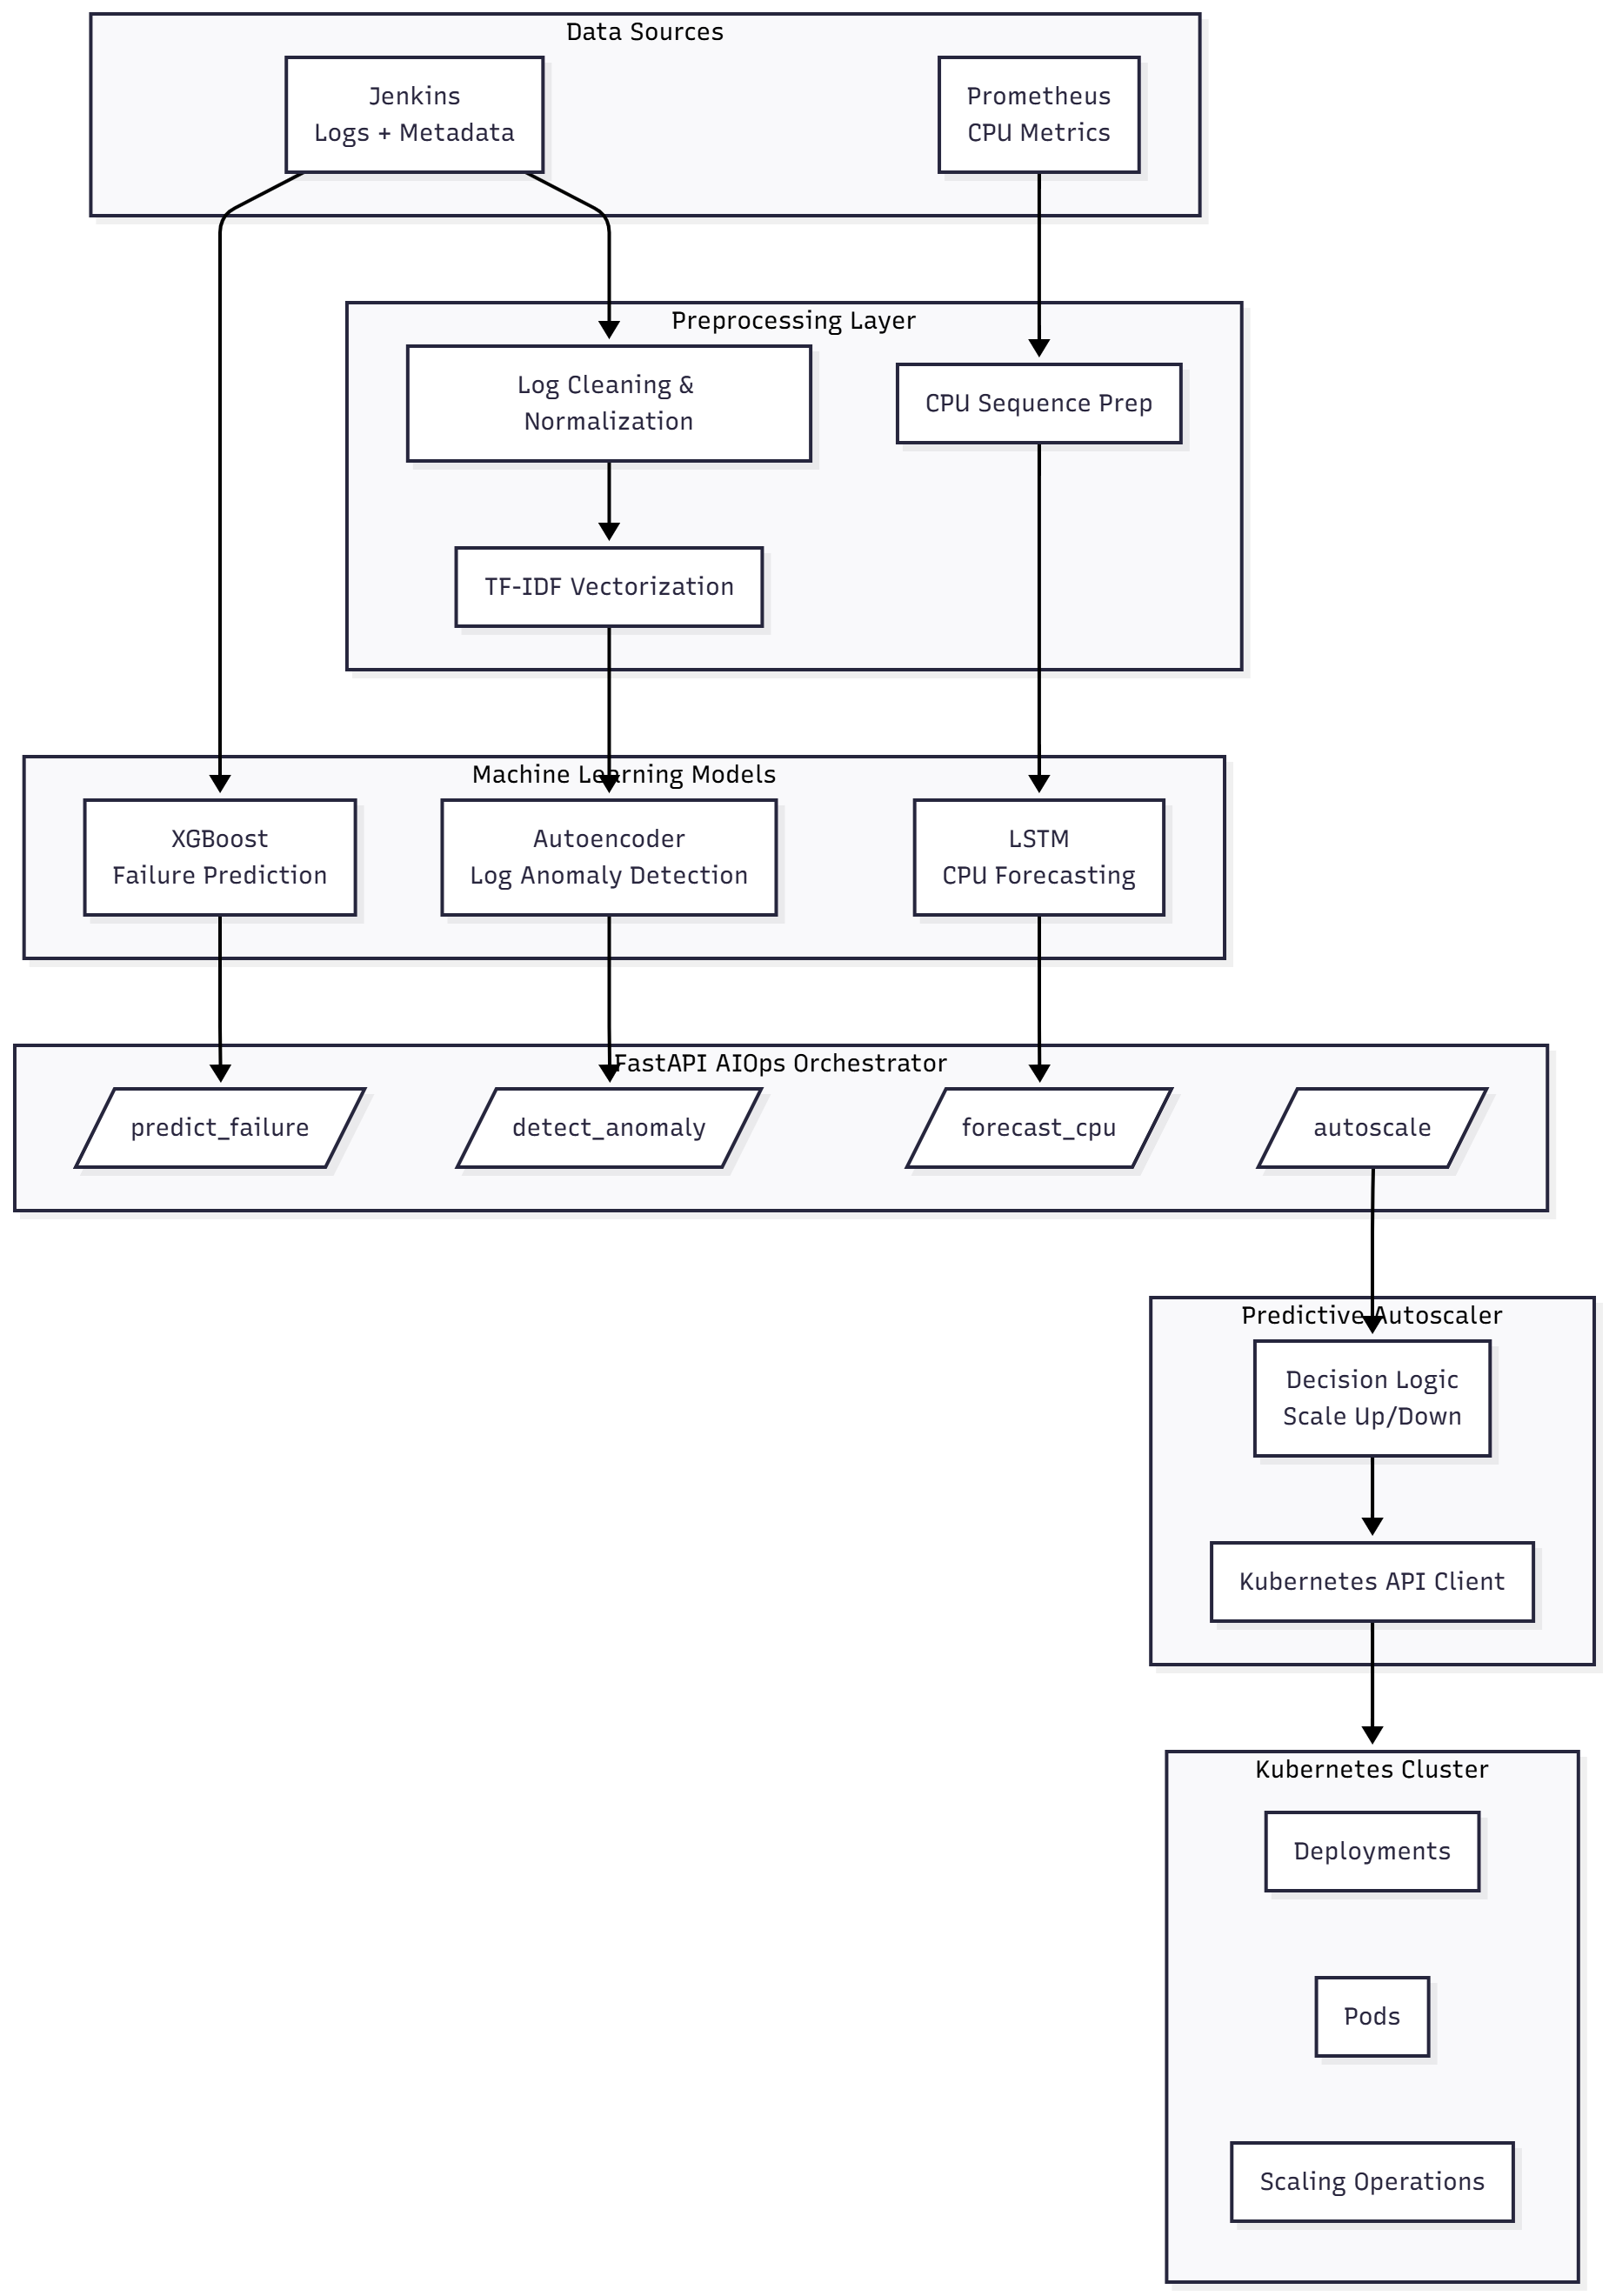
\includegraphics[width=0.9\textwidth]{architecutre.png}
    \caption{System Architecture Showing Data Flow from CI/CD to ML Pipelines and Autoscaler}
    \label{fig:system_architecture}
\end{figure}

\section{Machine Learning Model Design}

All three machine learning models were designed as standalone components with clear preprocessing, training, evaluation, and serialization stages.

\subsection{XGBoost Failure Prediction Model}

The XGBoost classifier is designed to predict whether a CI/CD build will fail before execution, using structured Jenkins build metadata.

\begin{itemize}
    \item \textbf{Input Features:} duration, warnings, errors, failures, log\_length, tests\_failed, tests\_passed, tests\_total (8 features total).
    \item \textbf{Target Variable:} Binary classification: 1 for FAILURE, 0 for non-failure (SUCCESS/UNSTABLE).
\end{itemize}

\subsection{TF--IDF + Autoencoder Log Anomaly Detection Model}

The anomaly detection model uses a two-stage pipeline: TF--IDF vectorization of Jenkins console logs followed by a PyTorch Autoencoder for reconstruction-based anomaly detection.

\begin{itemize}
    \item \textbf{Text Vectorization:} TF--IDF vectorizer with 500 features, n-gram range (1, 2), sublinear TF scaling, and English stop-word removal.
    \item \textbf{Autoencoder Architecture (PyTorch):} Encoder Linear(500$\rightarrow$128) $\rightarrow$ ReLU $\rightarrow$ BatchNorm $\rightarrow$ Dropout(0.3) $\rightarrow$ Linear(128$\rightarrow$64) $\rightarrow$ ReLU $\rightarrow$ BatchNorm $\rightarrow$ Dropout(0.3) $\rightarrow$ Linear(64$\rightarrow$32) $\rightarrow$ ReLU (bottleneck). Decoder Linear(32$\rightarrow$64) $\rightarrow$ ReLU $\rightarrow$ BatchNorm $\rightarrow$ Dropout(0.3) $\rightarrow$ Linear(64$\rightarrow$128) $\rightarrow$ ReLU $\rightarrow$ BatchNorm $\rightarrow$ Dropout(0.3) $\rightarrow$ Linear(128$\rightarrow$500) $\rightarrow$ Sigmoid.
    \item \textbf{Anomaly Threshold:} Determined at the 95th percentile of reconstruction errors on the normal training data. A log is flagged as anomalous when its reconstruction error exceeds this threshold.
\end{itemize}

\subsection{LSTM CPU Forecasting Model}

The LSTM model is designed to forecast future CPU usage from Prometheus time-series data.

\begin{itemize}
    \item \textbf{Sequence Design:} Sliding-window sequences with a lookback of 60 minutes and a forecast horizon of 10 minutes.
    \item \textbf{LSTM Architecture (PyTorch):} LSTM(input=1, hidden=128, batch\_first) $\rightarrow$ Dropout(0.2) $\rightarrow$ LSTM(128$\rightarrow$64) $\rightarrow$ Dropout(0.2) $\rightarrow$ Linear(64$\rightarrow$32) $\rightarrow$ ReLU $\rightarrow$ Linear(32$\rightarrow$1).
\end{itemize}

\section{Predictive Autoscaling Decision Policy}

The predictive autoscaler fuses the three ML signals predicted CPU, anomaly score, and failure probability using a priority-ordered policy, summarized in Table~\ref{alg:autoscale}.

\begin{table}[H]
\centering
\caption{Predictive Autoscaler Decision Policy}
\label{alg:autoscale}
\begin{tabular}{|p{1cm}|p{12.5cm}|}
\hline
\textbf{Step} & \textbf{Rule} \\
\hline
1 & If anomaly score $>$ anomaly threshold $\Rightarrow$ raise a non-blocking \emph{alert}. \\
\hline
2 & If failure probability $>$ 0.6 $\Rightarrow$ \emph{HOLD} (do not scale a likely-failing build). \\
\hline
3 & Else if predicted CPU $\geq$ 0.7 and replicas $<$ max $\Rightarrow$ \emph{scale up} by $+2$. \\
\hline
4 & Else if predicted CPU $\leq$ 0.3 and replicas $>$ min $\Rightarrow$ \emph{scale down} by $-1$. \\
\hline
5 & Otherwise $\Rightarrow$ \emph{maintain} current replicas. \\
\hline
\end{tabular}
\end{table}

The policy enforces operational safety constraints: a configurable replica range (default min = 1, max = 10), a cooldown period (default 300 s) that prevents oscillation by suppressing repeated scaling actions, and bounded per-action increments. Unlike the default Kubernetes HPA, which reacts only after measured CPU has already crossed a threshold, this policy acts on a \emph{forecast} of CPU ten minutes ahead and additionally vetoes scaling during likely-failing builds.

%_____________________________________________________________________________________________
\chapter{Experimental Setup}
%_____________________________________________________________________________________________

This chapter describes the hardware and software environment, the datasets and data collection infrastructure, the model training configuration, and the implementation of the orchestrator, autoscaler, and containerized deployment. The implementation was carried out on a Windows environment using Python 3.10+, with PyTorch for the deep-learning models (Autoencoder and LSTM) and XGBoost for the classification task. All trained artifacts are serialized into \texttt{orchestrator/models/} so that the orchestrator can load them at startup.

\section{Hardware Requirements}

The hardware requirements for the system are primarily driven by the computational needs of training machine learning models and running the AIOps orchestrator. The following configurations are recommended:

\subsection{Minimum Hardware Requirements}
\begin{itemize}
    \item \textbf{Processor:} Intel i5 (8th generation or higher) / AMD equivalent
    \item \textbf{Memory (RAM):} 8 GB
    \item \textbf{Storage:} 50 GB of free disk space
    \item \textbf{GPU:} Not mandatory; the models train on CPU, though a GPU accelerates Autoencoder and LSTM training
\end{itemize}

\subsection{Recommended Hardware Requirements}
\begin{itemize}
    \item \textbf{Processor:} Intel i7/i9, AMD Ryzen 7 or above
    \item \textbf{Memory (RAM):} 16--32 GB, to support parallel feature extraction and model training
    \item \textbf{Storage:} 100--250 GB SSD (for datasets, model checkpoints, logs)
    \item \textbf{GPU:} NVIDIA CUDA-enabled GPU (4--8 GB VRAM) for faster training of the Autoencoder and LSTM
\end{itemize}

\section{Software Requirements}

The software stack consists of operating system support, programming languages, libraries, and containerization environments required to implement the AIOps framework.

\subsection{Operating System}
\begin{itemize}
    \item Windows 10/11 (for development and experimentation)
    \item Linux-based system (Ubuntu 20.04 or later) for running Kubernetes clusters
\end{itemize}

\subsection{Programming Languages and Frameworks}
\begin{itemize}
    \item \textbf{Python 3.10+}: Core implementation language for ML models, collectors, and orchestrator.
    \item \textbf{FastAPI}: Framework for building the AIOps Orchestrator REST API.
    \item \textbf{PyTorch}: For implementing and training the Autoencoder and LSTM deep-learning models.
    \item \textbf{XGBoost}: For build failure prediction.
    \item \textbf{Scikit-learn}: For preprocessing, TF--IDF vectorization, train/test splitting, and evaluation metrics.
\end{itemize}

\subsection{Libraries and Dependencies}
\begin{itemize}
    \item NumPy, Pandas (data processing)
    \item Matplotlib (evaluation plots and visualization)
    \item Joblib (serialization of the XGBoost model, TF--IDF vectorizer, scaler, and threshold)
    \item Pydantic (FastAPI request/response models)
    \item Uvicorn (ASGI server)
    \item Kubernetes Python client (autoscaler scaling actions)
    \item Requests / python-jenkins (Jenkins and Prometheus HTTP access)
    \item python-dotenv (environment variables)
\end{itemize}

\subsection{External Services}
\begin{itemize}
    \item \textbf{Jenkins}: Source of CI/CD logs and build metadata
    \item \textbf{Prometheus}: Source of CPU and system metrics
    \item \textbf{Kubernetes API Server}: Used by the autoscaler for applying scaling actions
\end{itemize}

\section{Tools and Technology}

The development and deployment of the AIOps framework require a combination of DevOps, ML, and containerization tools. The following tools and technologies are used:

\begin{itemize}
    \item \textbf{Visual Studio Code}: Primary IDE for development.
    \item \textbf{Docker}: Containerization of the orchestrator and autoscaler components.
    \item \textbf{Minikube / Kubernetes Cluster}: Deployment and testing of the predictive autoscaler.
    \item \textbf{Prometheus \& Grafana}: Metric collection and monitoring dashboards.
    \item \textbf{GitHub}: Version control and collaborative code management.
    \item \textbf{Jenkins}: CI/CD tool providing logs and build metadata.
    \item \textbf{Python Kubernetes Client}: For implementing the custom autoscaling logic.
    \item \textbf{Postman / Curl}: For testing the FastAPI endpoints during development.
\end{itemize}

\section{Dataset Preparation}

\subsection{Synthetic Data Generation}

Since real-world CI/CD data from Jenkins and Prometheus was limited in volume, a comprehensive synthetic data generation module was developed to produce training-ready datasets that closely mimic production CI/CD environments. The data generator produces three categories of synthetic data:

\begin{itemize}
    \item \textbf{Jenkins Build Metadata:} 600 synthetic build records were generated with realistic distributions across SUCCESS ($\sim$68\%), FAILURE ($\sim$23\%), and UNSTABLE ($\sim$9\%) outcomes. Each record includes features such as duration, number of warnings, errors, test results (failed, passed, total), and log length. Feature correlations were carefully designed for example, failed builds tend to have longer durations, more errors, and more test failures.

    \item \textbf{Jenkins Console Logs:} 600 synthetic log files were generated using realistic templates that replicate actual Jenkins pipeline output. Logs include stages such as checkout, dependency installation, linting, testing, and build steps. Failure and success logs have distinct vocabulary patterns, making them suitable for anomaly detection training with TF--IDF vectorization.

    \item \textbf{Prometheus CPU Time-Series:} 10,080 CPU usage data points were generated as a time-series with realistic patterns including diurnal cycles, random spikes, gradual trends, and noise. This dataset was used for training the LSTM forecasting model with a sliding-window approach.
\end{itemize}

\subsection{Data Collection Infrastructure}

In addition to synthetic data, a complete data collection infrastructure was implemented to enable integration with live Jenkins and Prometheus instances:

\begin{itemize}
    \item \textbf{Jenkins Collector} (\texttt{collectors/jenkins\_collector.py}): A Python module that connects to Jenkins via its REST API using HTTP Basic Authentication. It retrieves build metadata (result, duration, timestamp), console logs, and test reports for specified jobs. Collected data is stored as structured CSVs and individual log files.

    \item \textbf{Prometheus Collector} (\texttt{collectors/prometheus\_collector.py}): A module that queries the Prometheus HTTP API to fetch time-series metrics such as CPU utilization, memory usage, and pod replica counts. It supports both instant and range queries using PromQL and exports results in structured CSV format.

    \item \textbf{Real-Time Collector} (\texttt{collectors/realtime\_collector.py}): A streaming collector designed for continuous, near-real-time data ingestion from both Jenkins and Prometheus sources.
\end{itemize}

A demonstration Next.js Todo application is included as the CI/CD target. It exposes a Prometheus-format metrics endpoint (\texttt{/api/metrics}) and ships with a Jenkinsfile defining a six-stage pipeline (Checkout $\rightarrow$ Install $\rightarrow$ Lint $\rightarrow$ Test $\rightarrow$ Build $\rightarrow$ Archive), enabling the framework to be exercised against a live build and monitoring environment.

\section{Model Training Configuration}

\subsection{XGBoost Failure Prediction Model}

The XGBoost classifier (\texttt{training/train\_failure\_xgboost.py}) was trained on Jenkins build metadata:

\begin{itemize}
    \item \textbf{Train/Test Split:} 80\%/20\% stratified split with random seed 42.
    \item \textbf{Hyperparameters:} 100 estimators, max depth 6, learning rate 0.1, subsample 0.8, colsample\_bytree 0.8, with automatic class-weight balancing via \texttt{scale\_pos\_weight}.
    \item \textbf{Output:} Trained model saved as \texttt{orchestrator/models/xgboost\_failure.bin}.
\end{itemize}

\subsection{TF--IDF + Autoencoder Log Anomaly Detection Model}

The anomaly detection model (\texttt{training/train\_log\_anomaly.py}) was trained as follows:

\begin{itemize}
    \item \textbf{Training:} Trained only on normal (non-anomalous) logs using MSE reconstruction loss with the Adam optimizer (lr = 0.0005).
    \item \textbf{Output:} TF--IDF vectorizer (\texttt{tfidf.pkl}), Autoencoder weights (\texttt{autoencoder.pth}), and threshold (\texttt{anomaly\_threshold.pkl}) saved to \texttt{orchestrator/models/}.
\end{itemize}

\subsection{LSTM CPU Forecasting Model}

The LSTM model (\texttt{training/train\_cpu\_lstm.py}) was trained on the Prometheus CPU time-series:

\begin{itemize}
    \item \textbf{Data Preprocessing:} CPU values normalized to [0, 1] using a MinMaxScaler. Sliding-window sequences were created with a lookback of 60 minutes and a forecast horizon of 10 minutes, yielding 10,011 training sequences.
    \item \textbf{Training:} MSE loss with the Adam optimizer (lr = 0.001), batch size 32, and learning-rate reduction on plateau (factor 0.5, patience 5).
    \item \textbf{Output:} LSTM weights (\texttt{lstm\_cpu.pth}) and the scaler (\texttt{cpu\_scaler.pkl}) saved to \texttt{orchestrator/models/}.
\end{itemize}

\section{FastAPI AIOps Orchestrator}

The orchestrator (\texttt{orchestrator/main.py}) is the central inference layer that unifies all three models behind a single REST interface. It is implemented using FastAPI with an asynchronous lifespan handler that loads every model into memory once at startup, so that subsequent inference requests are served without reloading. The application is organized into modular routers, one per capability, and a set of utility modules for Kubernetes and Prometheus access.

\begin{table}[H]
\centering
\caption{AIOps Orchestrator: REST API Endpoints}
\label{table:api_endpoints}
\begin{tabular}{|l|l|p{6.2cm}|}
\hline
\textbf{Endpoint} & \textbf{Method} & \textbf{Description} \\
\hline
\texttt{/} & GET & Service information and available endpoints \\
\hline
\texttt{/health} & GET & Liveness/health check \\
\hline
\texttt{/predict\_failure} & POST & Returns build failure probability (XGBoost) \\
\hline
\texttt{/detect\_anomaly} & POST & Returns anomaly score and boolean flag (Autoencoder) \\
\hline
\texttt{/forecast\_cpu} & POST & Returns predicted CPU usage from history (LSTM) \\
\hline
\texttt{/autoscale} & POST & Triggers the predictive autoscaling decision \\
\hline
\end{tabular}
\end{table}

Each endpoint uses Pydantic models for request and response validation. Interactive Swagger documentation is automatically served at \texttt{/docs}. A representative request and response for the failure-prediction endpoint is shown below:

\begin{lstlisting}
POST /predict_failure
{
  "duration": 120, "warnings": 5, "errors": 8, "failures": 2,
  "log_length": 25000, "tests_failed": 5,
  "tests_passed": 19, "tests_total": 24
}
-> { "failure_probability": 0.974 }
\end{lstlisting}

\section{Predictive Autoscaler Implementation}

The predictive autoscaler is implemented in two parts: a \texttt{DecisionEngine} (\texttt{autoscaler/decision\_engine.py}) that encapsulates the scaling policy of Table~\ref{alg:autoscale}, and a \texttt{PredictiveScaler} (\texttt{autoscaler/scaler.py}) that applies decisions to a Kubernetes deployment using the Kubernetes Python client.

The engine enforces operational safety constraints: a configurable replica range (default min = 1, max = 10), a cooldown period (default 300 s) that prevents oscillation by suppressing repeated scaling actions, and bounded per-action increments. The \texttt{PredictiveScaler} reads the current replica count from the cluster, invokes the decision engine, and patches the deployment's replica count only when a scaling action is warranted. If no Kubernetes cluster is reachable, the orchestrator degrades gracefully the other three endpoints remain fully functional while \texttt{/autoscale} reports that the cluster is unavailable.

\section{Containerization and Kubernetes Deployment}

The orchestrator and autoscaler are containerized using a single Dockerfile based on the \texttt{python:3.11-slim} image. The image installs the Python dependencies, copies the application code together with the trained model artifacts, exposes port 8000, and launches the service through Uvicorn. Kubernetes manifests are provided in \texttt{kubernetes\_manifests/}:

\begin{itemize}
    \item \texttt{orchestrator-deployment.yaml}: Deployment for the AIOps orchestrator.
    \item \texttt{autoscaler-deployment.yaml}: Deployment for the predictive autoscaler, including the ServiceAccount/RBAC needed to patch deployment replicas.
    \item \texttt{demo-app-deployment.yaml}: Deployment for the demo Todo application that acts as the scaling target.
    \item \texttt{service.yaml}: Service exposing the orchestrator within the cluster.
\end{itemize}

A PowerShell helper (\texttt{scripts/deploy-minikube.ps1}) automates building the image into the Minikube Docker context and applying the manifests, enabling single-command local deployment.

%_____________________________________________________________________________________________
\chapter{Results and Discussion}
%_____________________________________________________________________________________________

A comprehensive evaluation suite (\texttt{evaluation/evaluate\_all.py}) loads the trained models, computes standard metrics on held-out test data, and generates twelve publication-quality plots together with a consolidated metrics report (\texttt{evaluation/metrics/all\_metrics.json}). This chapter reports those results, followed by the behaviour of the predictive autoscaler.

\section{XGBoost Failure Prediction Results}

The XGBoost model demonstrated excellent performance on the 20\% held-out test set:

\begin{table}[H]
\centering
\caption{XGBoost Failure Prediction: Test Set Performance}
\label{table:xgboost_results}
\begin{tabular}{|l|c|}
\hline
\textbf{Metric} & \textbf{Value} \\
\hline
Accuracy & 99.17\% \\
Precision & 96.43\% \\
Recall & 100.00\% \\
F1-Score & 98.18\% \\
\hline
\end{tabular}
\end{table}

A 5-fold stratified cross-validation was also performed to verify model stability:

\begin{table}[H]
\centering
\caption{XGBoost 5-Fold Cross-Validation Results}
\label{table:xgboost_cv}
\begin{tabular}{|l|c|}
\hline
\textbf{Metric} & \textbf{Mean $\pm$ Std} \\
\hline
Accuracy & 99.00\% $\pm$ 0.62\% \\
F1-Score & 97.83\% $\pm$ 1.37\% \\
\hline
\end{tabular}
\end{table}

The low cross-validation variance confirms that the model generalizes consistently across folds rather than relying on a favourable single split. The feature importance analysis revealed that \texttt{errors}, \texttt{failures}, and \texttt{tests\_failed} were the most influential predictors of build failure, which is intuitive from a DevOps standpoint.

\begin{figure}[H]
    \centering
    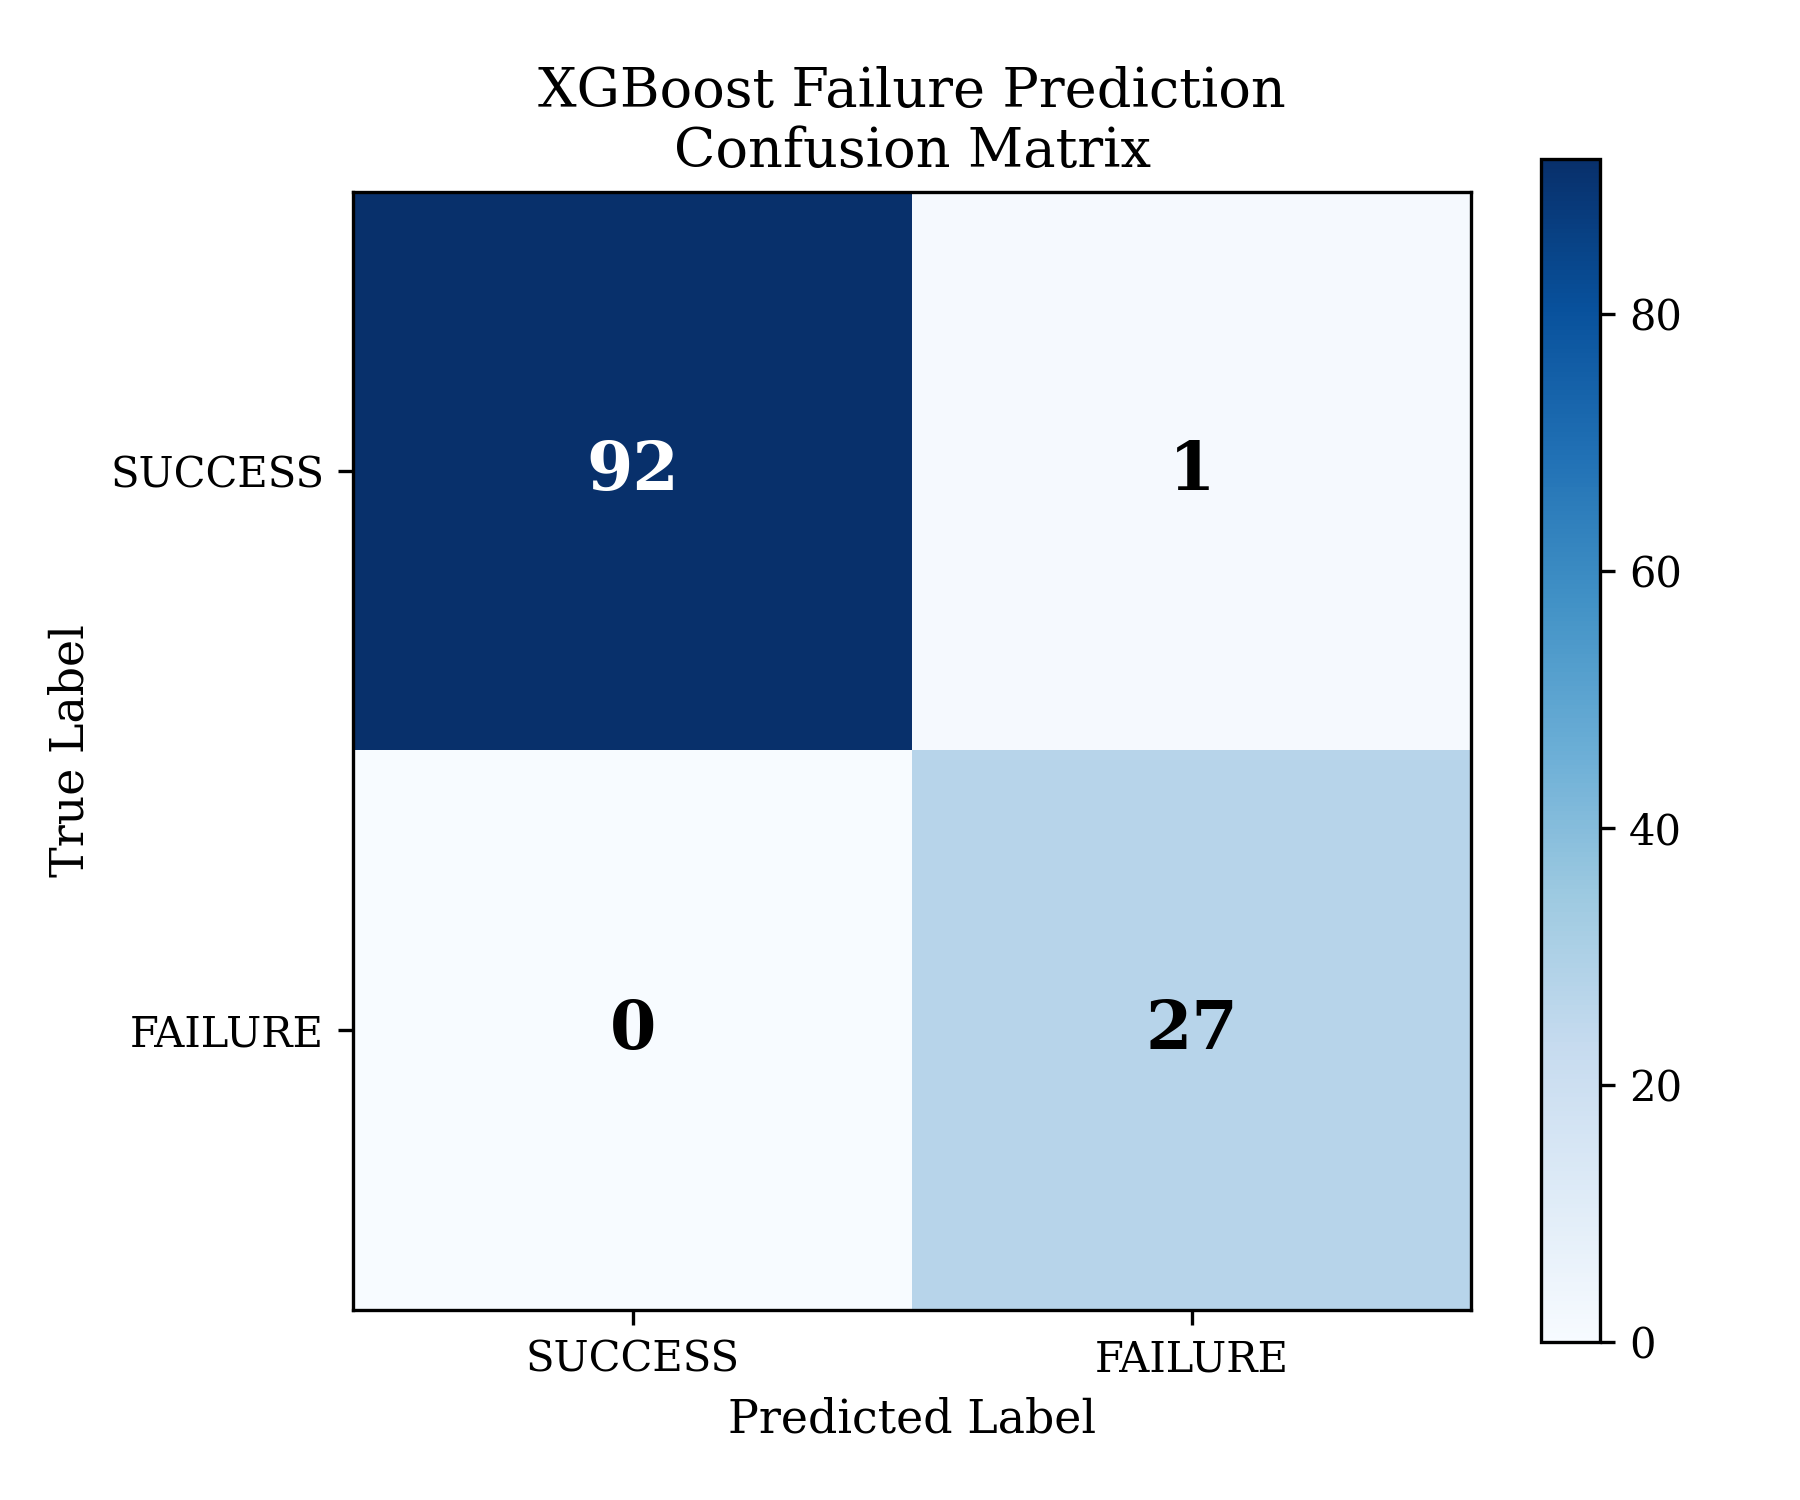
\includegraphics[width=0.55\textwidth]{xgboost_confusion_matrix.png}
    \caption{XGBoost Failure Prediction: Confusion Matrix}
    \label{fig:xgb_cm}
\end{figure}

\begin{figure}[H]
    \centering
    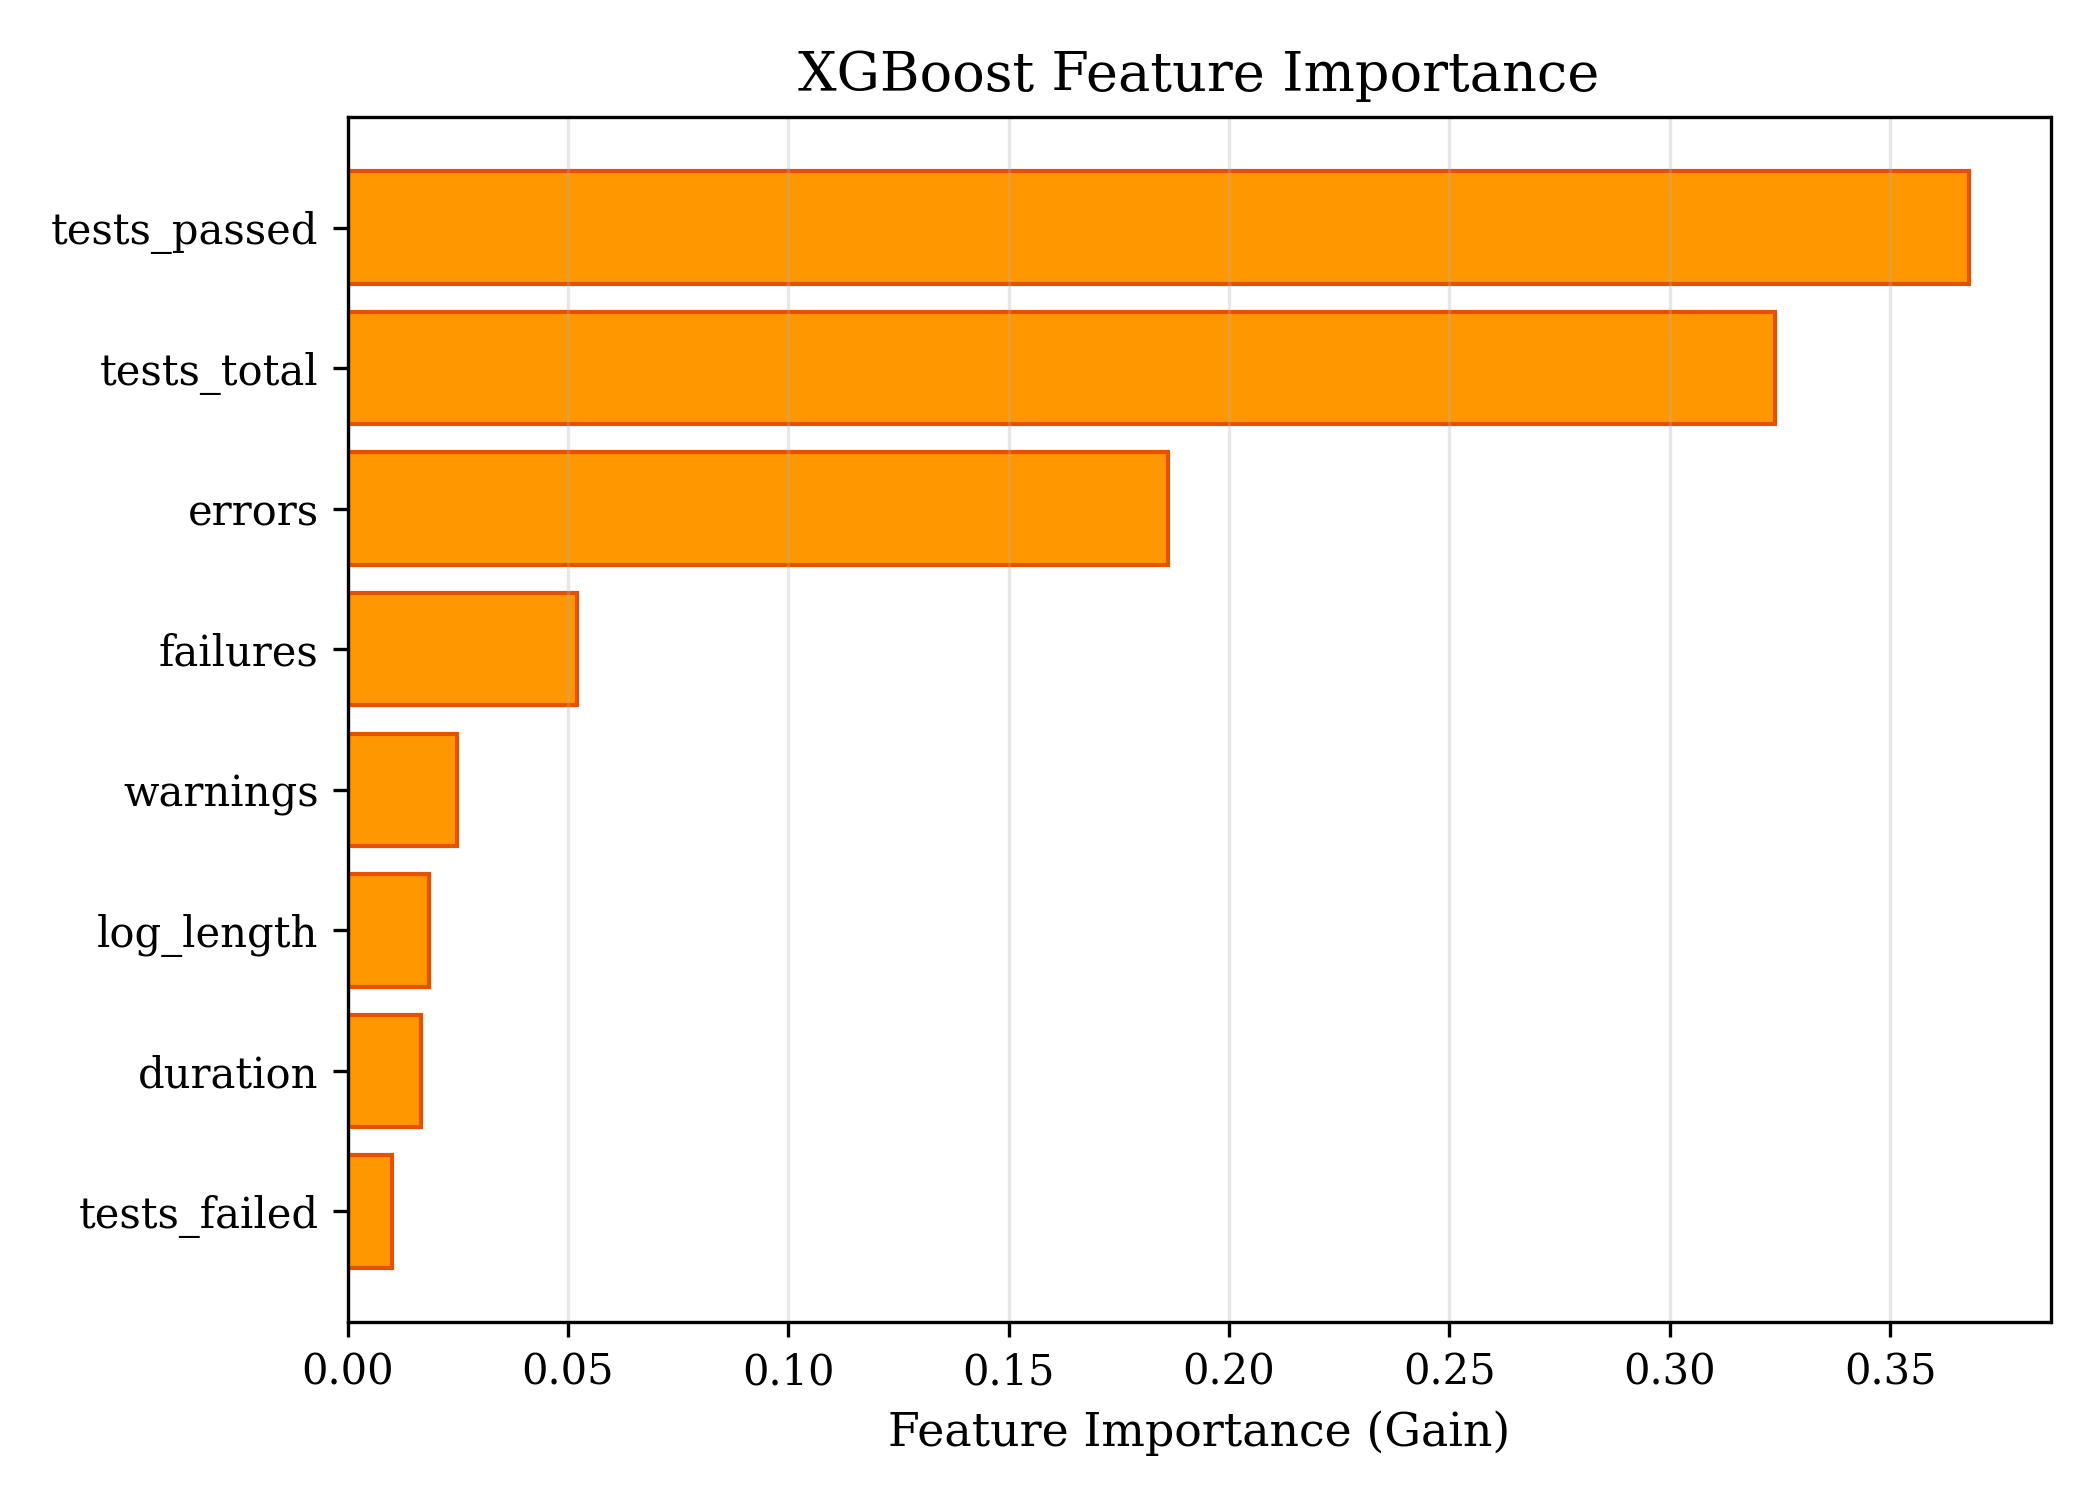
\includegraphics[width=0.60\textwidth]{xgboost_feature_importance.png}
    \caption{XGBoost Feature Importance Analysis}
    \label{fig:xgb_fi}
\end{figure}

\section{Anomaly Detection Results}

The TF--IDF + Autoencoder anomaly detector was evaluated on a held-out test set drawn from the 600 console logs:

\begin{table}[H]
\centering
\caption{Log Anomaly Detection: Test Set Performance}
\label{table:anomaly_results}
\begin{tabular}{|l|c|}
\hline
\textbf{Metric} & \textbf{Value} \\
\hline
Accuracy & 96.67\% \\
Precision & 87.10\% \\
Recall & 100.00\% \\
F1-Score & 93.10\% \\
\hline
\end{tabular}
\end{table}

The model achieved perfect recall (100\%), meaning it detected every anomalous (failure) log in the test set an important property for an operational alerting system, where missing a genuine anomaly is far more costly than a false alarm. The reconstruction-error distribution (Figure~\ref{fig:anomaly_dist}) shows a clear separation between normal and anomalous logs around the learned 95th-percentile threshold. It should be noted that, because the evaluation uses synthetic logs in which failure and success messages have distinctive vocabulary, the class separability is high; on noisier real-world logs the precision would be expected to decrease, and threshold calibration on live data is identified as part of the future scope.

\begin{figure}[H]
    \centering
    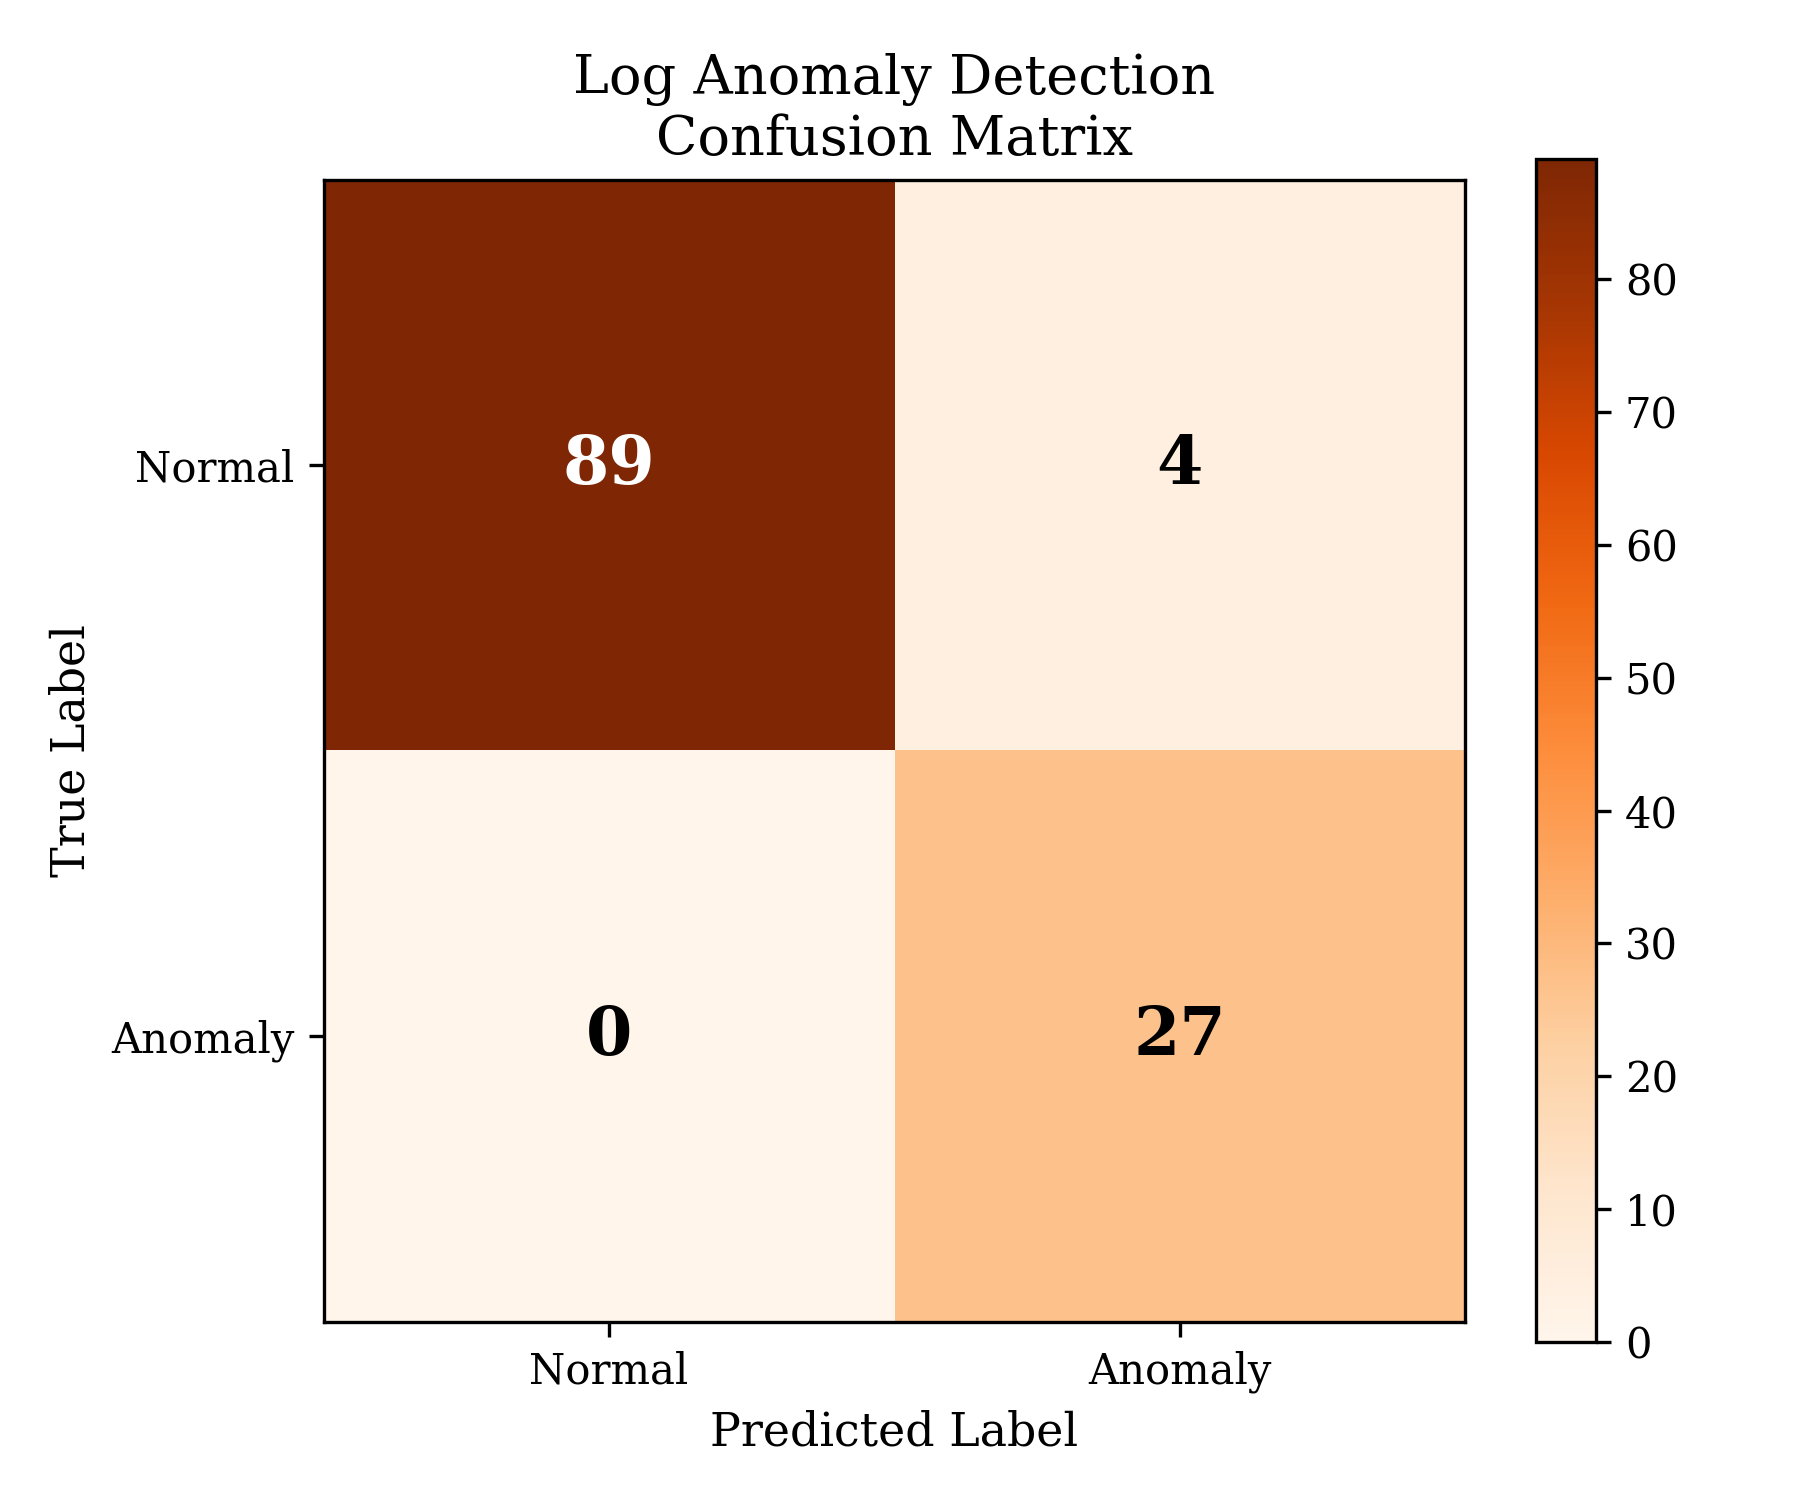
\includegraphics[width=0.55\textwidth]{anomaly_confusion_matrix.png}
    \caption{Log Anomaly Detection: Confusion Matrix}
    \label{fig:anomaly_cm}
\end{figure}

\begin{figure}[H]
    \centering
    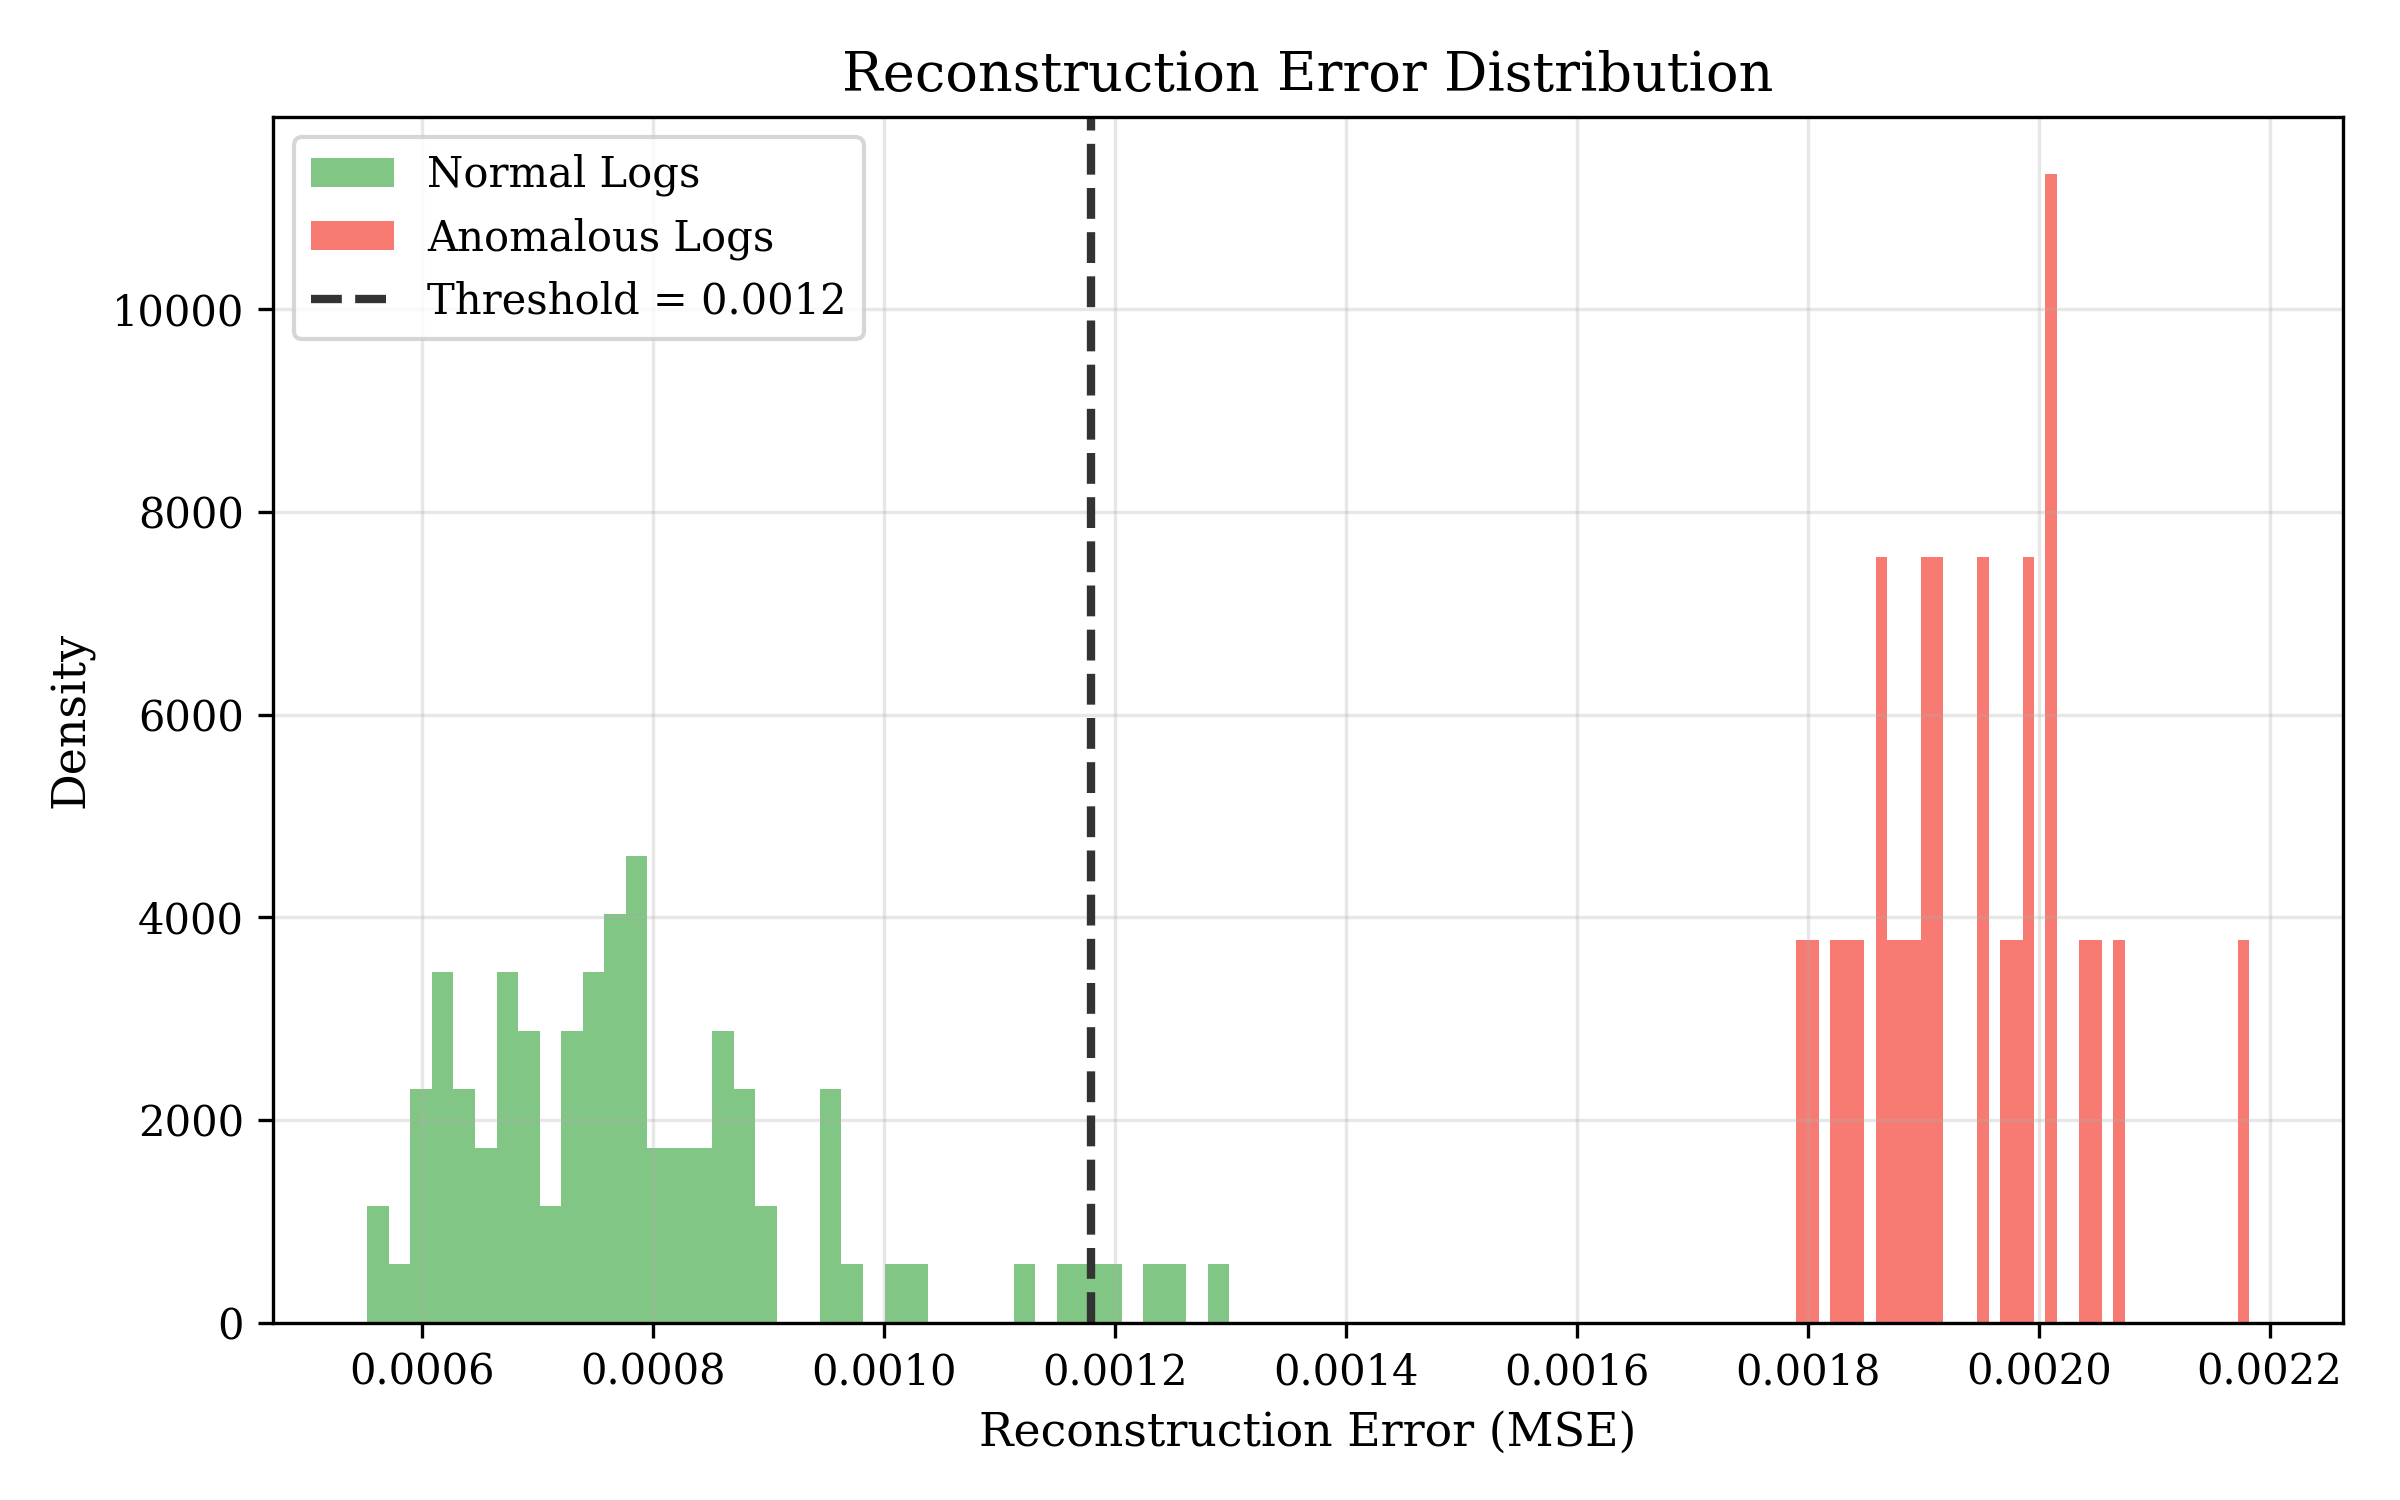
\includegraphics[width=0.65\textwidth]{anomaly_error_distribution.png}
    \caption{Reconstruction Error Distribution: Normal vs Anomalous Logs}
    \label{fig:anomaly_dist}
\end{figure}

\section{LSTM CPU Forecasting Results}

The LSTM model was evaluated on the temporally held-out portion of the CPU time-series:

\begin{table}[H]
\centering
\caption{LSTM CPU Forecasting: Test Set Performance}
\label{table:lstm_results}
\begin{tabular}{|l|c|}
\hline
\textbf{Metric} & \textbf{Value} \\
\hline
MSE & 0.0049 \\
MAE & 0.0433 \\
RMSE & 0.0698 \\
MAPE & 9.68\% \\
R\textsuperscript{2} & 0.455 \\
\hline
\end{tabular}
\end{table}

The model demonstrates strong short-term forecasting capability, with a mean absolute error of roughly 4.3\% of the normalized CPU range and a MAPE under 10\%. The actual-vs-predicted overlay (Figure~\ref{fig:lstm_pred}) confirms that predictions closely track real CPU trends, and the residuals are approximately centred on zero. The moderate R\textsuperscript{2} reflects the substantial random-noise component deliberately injected into the synthetic series; the low RMSE/MAE confirm that the model captures the underlying diurnal and trend structure that matters for proactive scaling decisions.

\begin{figure}[H]
    \centering
    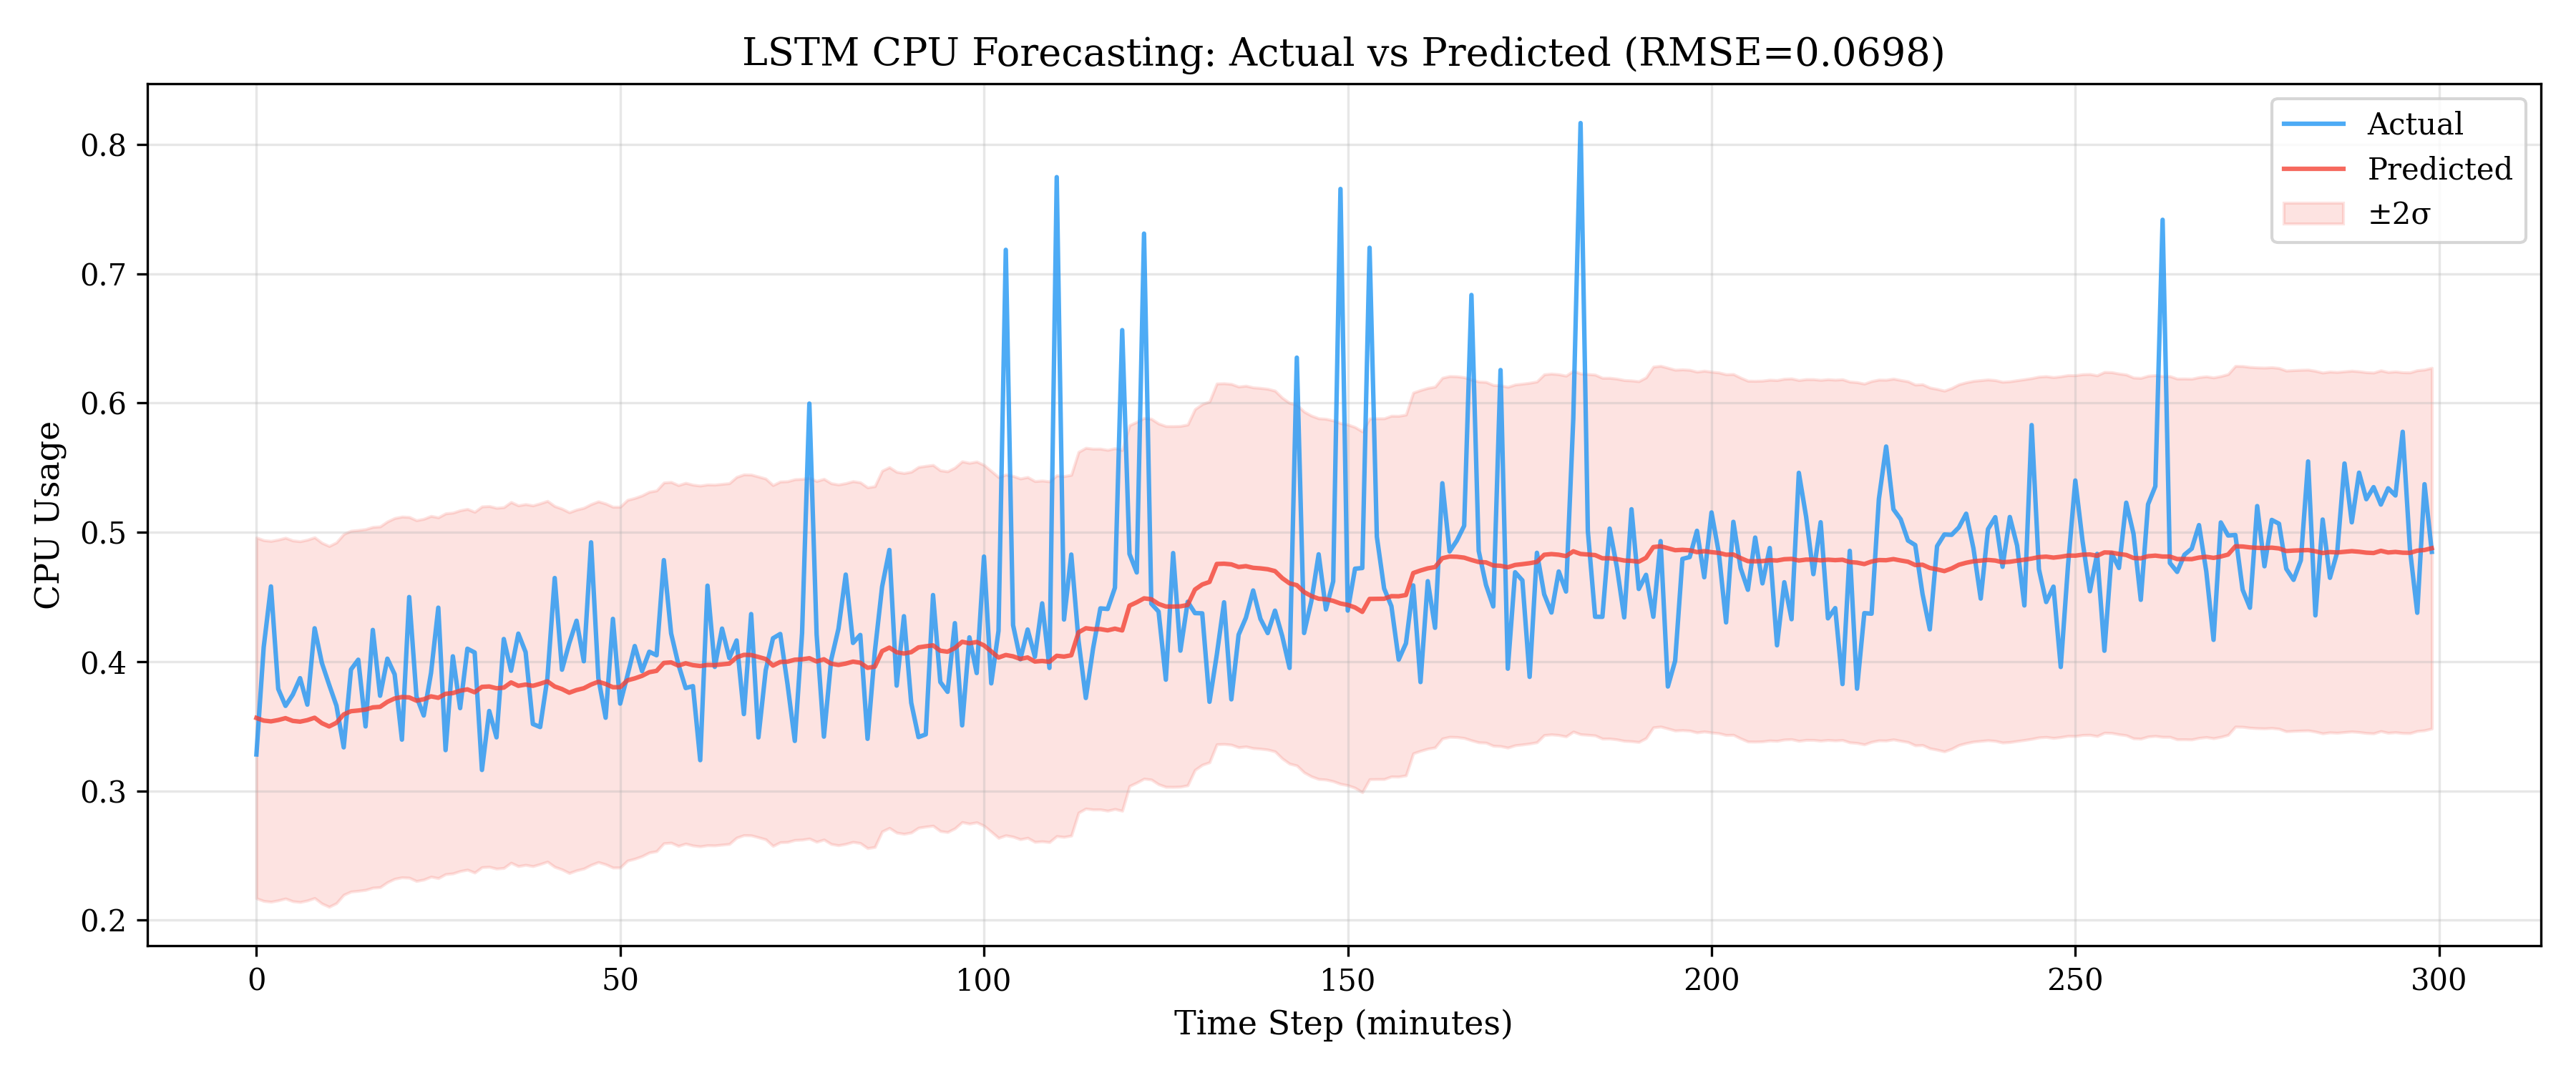
\includegraphics[width=0.75\textwidth]{lstm_actual_vs_predicted.png}
    \caption{LSTM CPU Forecasting: Actual vs Predicted Values}
    \label{fig:lstm_pred}
\end{figure}

\begin{figure}[H]
    \centering
    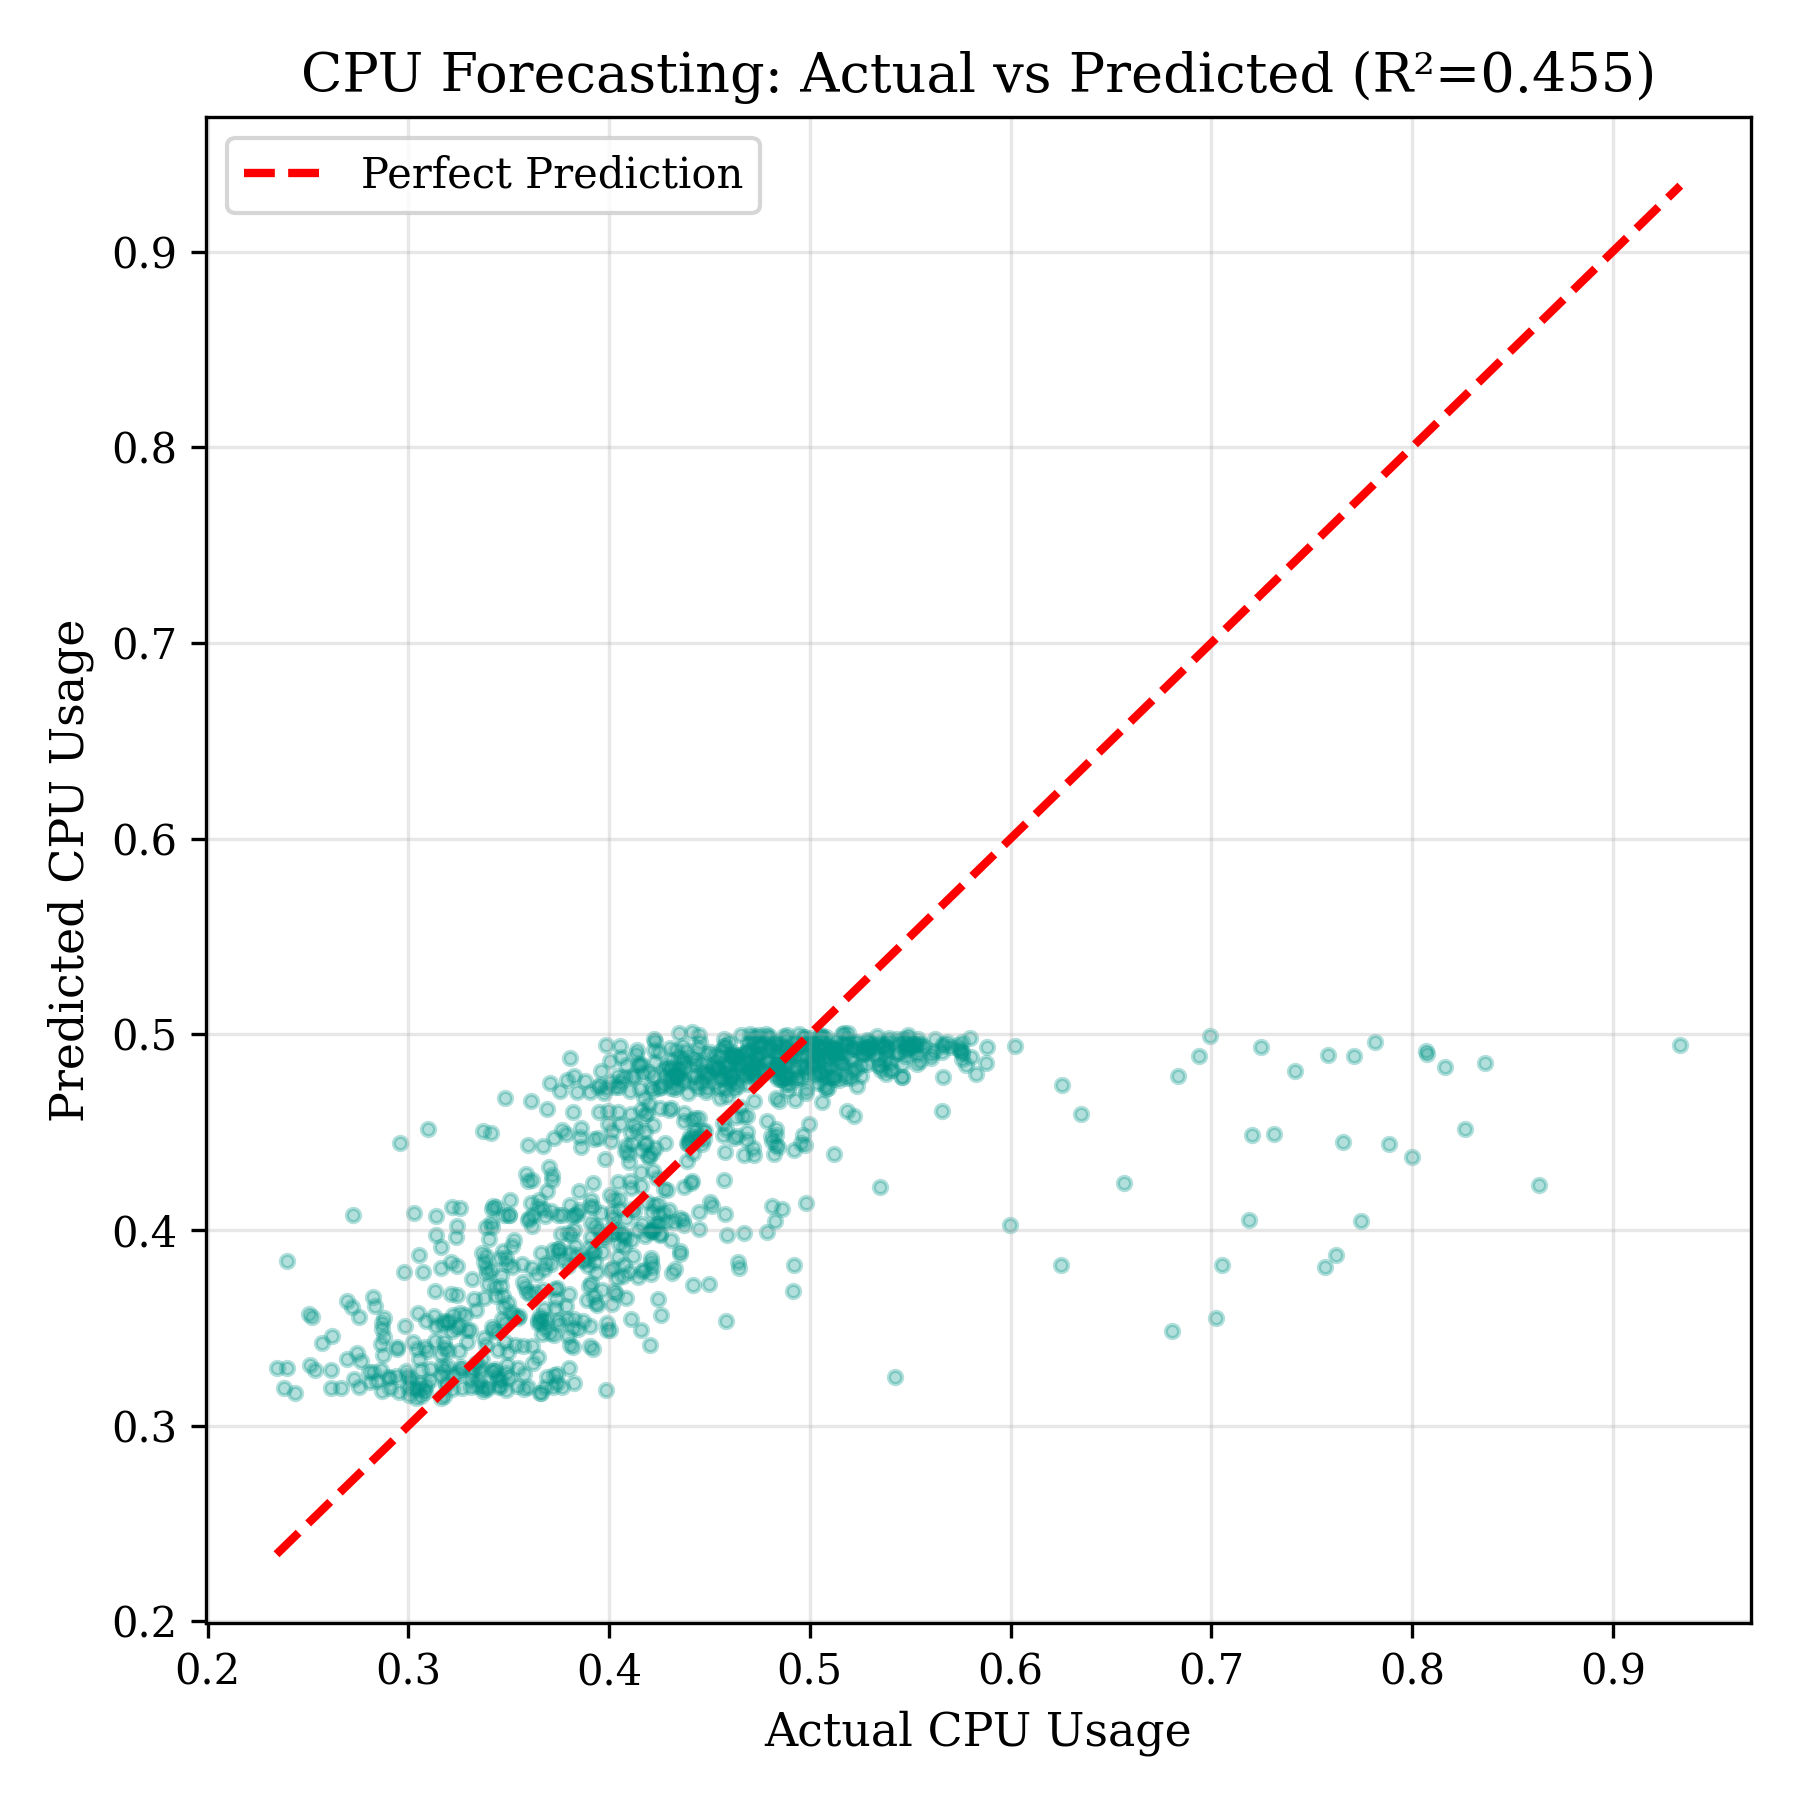
\includegraphics[width=0.50\textwidth]{lstm_scatter.png}
    \caption{LSTM CPU Forecasting: Actual vs Predicted Scatter Plot}
    \label{fig:lstm_scatter}
\end{figure}

\section{Combined Model Performance Summary}

Table~\ref{table:combined_summary} presents a consolidated view of all three model performances.

\begin{table}[H]
\centering
\caption{AIOps System: Combined Model Performance Summary}
\label{table:combined_summary}
\begin{tabular}{|p{3.5cm}|p{3.5cm}|p{3cm}|p{3cm}|}
\hline
\textbf{Module} & \textbf{Algorithm} & \textbf{Key Metric} & \textbf{ROC AUC / R\textsuperscript{2}} \\
\hline
Failure Prediction & XGBoost & F1 = 0.982 & AUC = 1.000 \\
\hline
Anomaly Detection & TF--IDF + Autoencoder & F1 = 0.931 & AUC = 1.000 \\
\hline
CPU Forecasting & LSTM & RMSE = 0.070 & R\textsuperscript{2} = 0.455 \\
\hline
\end{tabular}
\end{table}

\begin{figure}[H]
    \centering
    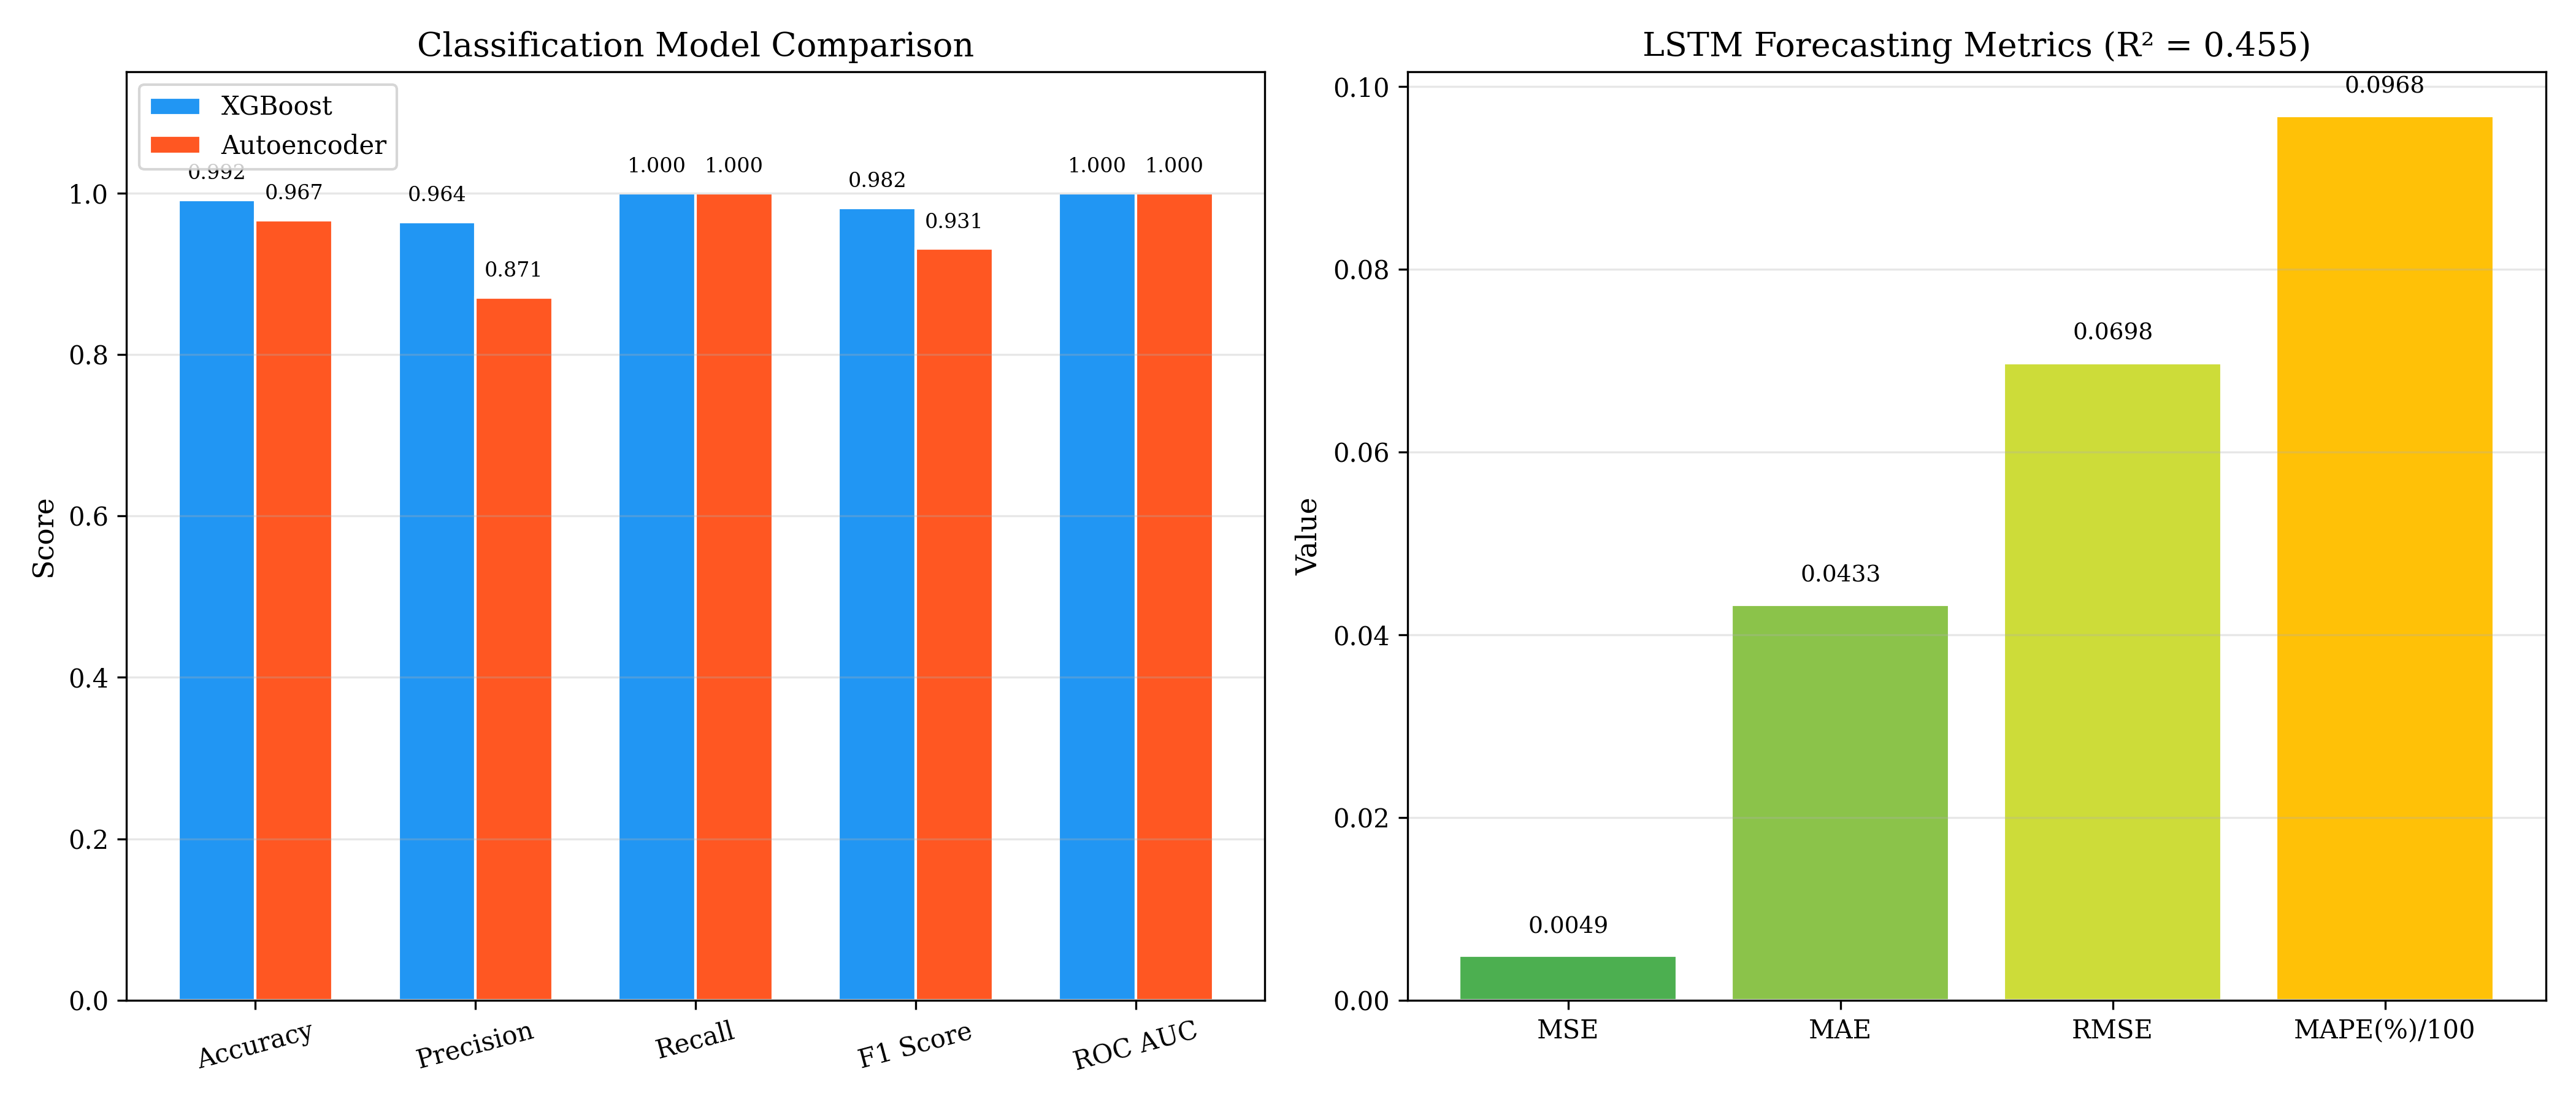
\includegraphics[width=0.80\textwidth]{model_comparison_summary.png}
    \caption{Model Comparison: Classification Metrics and Forecasting Metrics}
    \label{fig:model_comparison}
\end{figure}

\section{Predictive Autoscaler Behaviour}

The decision engine was exercised on a set of representative operating scenarios to verify that the fused-signal policy behaves correctly. Table~\ref{table:autoscale_results} reports the actual decisions produced by the implementation for a deployment currently running 5 replicas (with the at-maximum case starting from 10). The results confirm each branch of the decision policy in Table~\ref{alg:autoscale}: high forecast CPU triggers a proactive scale-up, low forecast CPU triggers a scale-down, a high failure probability holds scaling to avoid wasting resources on a failing build, a log anomaly raises an alert while still allowing CPU-driven scaling, and the replica ceiling is respected.

\begin{table}[H]
\centering
\caption{Predictive Autoscaler: Decisions for Representative Scenarios}
\label{table:autoscale_results}
\begin{tabular}{|p{4.3cm}|c|c|c|c|c|}
\hline
\textbf{Scenario} & \textbf{CPU} & \textbf{Anom.} & \textbf{Fail.} & \textbf{Action} & \textbf{Replicas} \\
\hline
High CPU forecast & 0.85 & 0.10 & 0.20 & scale\_up & 5 $\rightarrow$ 7 \\
\hline
Low CPU forecast & 0.20 & 0.05 & 0.10 & scale\_down & 5 $\rightarrow$ 4 \\
\hline
Normal load & 0.50 & 0.10 & 0.20 & no\_action & 5 \\
\hline
High failure prob. (hold) & 0.90 & 0.10 & 0.80 & no\_action & 5 \\
\hline
Anomaly + high CPU & 0.80 & 0.95 & 0.20 & scale\_up + alert & 5 $\rightarrow$ 7 \\
\hline
At maximum replicas & 0.95 & 0.10 & 0.20 & no\_action & 10 \\
\hline
\end{tabular}
\end{table}

Unlike the default Kubernetes HPA, which reacts only after measured CPU has already crossed a threshold, this engine acts on a \emph{forecast} of CPU ten minutes ahead and additionally vetoes scaling during likely-failing builds. This proactive, signal-fused behaviour is the central practical contribution of the framework.

\section{Summary of Implementation Outcomes}

The following outcomes were achieved:

\begin{itemize}
    \item Complete synthetic data generation pipeline for Jenkins builds, console logs, and CPU time-series, plus live Jenkins/Prometheus collectors.
    \item XGBoost failure-prediction model: 99.17\% accuracy, 98.18\% F1, 99.0\% mean CV accuracy.
    \item TF--IDF + Autoencoder anomaly detector: 96.67\% accuracy, 93.10\% F1, 100\% recall.
    \item LSTM CPU forecaster: RMSE 0.070, MAE 0.043, MAPE 9.68\%.
    \item All three models integrated into a FastAPI orchestrator that loads them at startup and serves real-time inference.
    \item A predictive autoscaler implemented with the Kubernetes Python client, fusing the three ML signals under a priority policy with cooldown and replica limits.
    \item Containerization (Docker) and Kubernetes manifests for the orchestrator, autoscaler, and demo application, with a one-command Minikube deployment script.
\end{itemize}

%_____________________________________________________________________________________________
\chapter{Conclusion and Future Work}
%_____________________________________________________________________________________________

\section{Conclusion}

This dissertation set out to replace reactive DevOps mechanisms with a proactive, data-driven AIOps framework, and it has achieved that goal end-to-end. Three machine learning models were designed, trained, and rigorously evaluated: an XGBoost classifier that predicts CI/CD build failures before execution, a TF--IDF + Autoencoder model that flags anomalous Jenkins console logs without requiring labelled anomalies, and an LSTM network that forecasts short-term Kubernetes CPU usage. On held-out test data the models attained 99.17\% accuracy (failure prediction), 96.67\% accuracy with perfect recall (anomaly detection), and an RMSE of 0.070 with a MAPE under 10\% (CPU forecasting).

Crucially, the work goes beyond isolated models. All three were unified behind a single FastAPI orchestrator that loads them at startup and serves real-time inference, and their outputs were fused by a predictive autoscaler that makes proactive Kubernetes scaling decisions while respecting cooldown intervals and replica limits. The entire pipeline from data ingestion through inference to autoscaling was containerized and deployed using Docker and Kubernetes manifests. In doing so, the dissertation directly addresses the central research gap identified in the literature: the absence of a single framework that combines failure prediction, log anomaly detection, and predictive autoscaling. The system demonstrates that fusing CI/CD signals with resource forecasts enables earlier, better-informed operational decisions than any of these signals could provide in isolation.

\section{Future Work}

While the framework is complete and functional, several directions would strengthen it for production use:

\begin{enumerate}
    \item \textbf{Validation on real-world data:} Replacing the synthetic datasets with logs and metrics collected from production Jenkins and Prometheus instances, and recalibrating the anomaly threshold on live traffic, to confirm the metrics generalize beyond the synthetic separability of the current logs.
    \item \textbf{Quantitative benchmarking against HPA:} Running controlled cluster experiments that compare the predictive autoscaler against the default Horizontal Pod Autoscaler on response time, SLA violations, and resource cost.
    \item \textbf{Stronger log models:} Evaluating transformer-based log encoders (e.g., LogBERT-style models) against the TF--IDF + Autoencoder baseline where compute permits, to capture sequence-level context.
    \item \textbf{Online / continual learning:} Periodically retraining the models on freshly collected data so that they adapt to drift in pipeline behaviour and workload patterns.
    \item \textbf{Monitoring dashboard:} A Grafana or Streamlit dashboard surfacing live predictions, anomaly alerts, CPU forecasts, and autoscaling actions, together with Prometheus-based alerting.
    \item \textbf{Closed-loop remediation:} Extending the autoscaler into a broader remediation engine that can, for example, automatically retry or quarantine builds predicted to fail.
\end{enumerate}

	% ---------- APPENDICES ----------
	\appendix

	\chapter{Publications}
	I am pleased to acknowledge that a part of this research work has been published in \textbf{ICICST-2026} (International Conference on Innovations in Computing, Communication, and Sustainable Technologies) under the title \textit{``A Systematic Review of AIOps Techniques for Failure Prediction and Resource Optimization in CI/CD Pipelines''}. I sincerely thank my guide, co-guide, and all the co-authors for their valuable contributions, constructive feedback, and support throughout the research and publication process.

\begin{figure}[H]
    \centering
    
\includegraphics[width=\textwidth]{icicst_website.png}
    \caption{ICICST-2026 Conference Website}
    \label{fig:icicst_website}
\end{figure}

\begin{figure}[H]
    \centering
    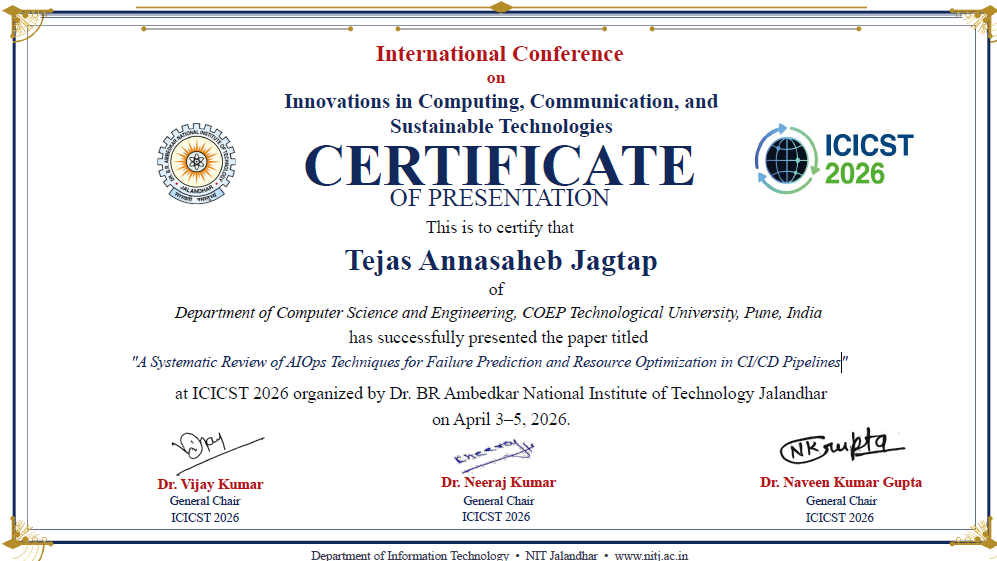
\includegraphics[width=\textwidth]{icicst_certificate.png}
    \caption{Certificate of Presentation -- ICICST-2026}
    \label{fig:icicst_certificate}
\end{figure}

	\clearpage

	\chapter{Timeline}
	% Adjust the activity dates below as per the actual project schedule.
	\begin{table}[H]
	\centering
	\caption{Dissertation Timeline}
	\label{table:timeline}
	\begin{tabular}{|p{4cm}|p{10cm}|}
	\hline
	\textbf{Duration} & \textbf{Activity} \\
	\hline
	Jul--Aug 2025 & Literature survey and problem formulation \\
	\hline
	Sep 2025 & Requirement analysis and high-level system design \\
	\hline
	Oct--Nov 2025 & Data collection infrastructure and synthetic dataset generation \\
	\hline
	Dec 2025 & XGBoost failure-prediction model development and evaluation \\
	\hline
	Jan 2026 & TF--IDF + Autoencoder log anomaly detection model \\
	\hline
	Feb 2026 & LSTM CPU forecasting model \\
	\hline
	Mar 2026 & FastAPI AIOps orchestrator integration \\
	\hline
	Apr 2026 & Predictive autoscaler and Kubernetes deployment \\
	\hline
	May 2026 & End-to-end evaluation and result analysis \\
	\hline
	Jun 2026 & Dissertation report writing and submission \\
	\hline
	\end{tabular}
	\end{table}
	\clearpage

	% ---------- REFERENCES ----------
	\renewcommand{\bibname}{References}
	\addcontentsline{toc}{chapter}{References}
	\nocite{*}
	\bibliographystyle{unsrt}
	\bibliography{bib/refs}
	\clearpage

\end{document}
